\documentclass{book}
\usepackage{titlesec}
\usepackage{hyperref}
\hypersetup{colorlinks}% uncomment this line if you prefer colored hyperlinks (e.g., for onscreen viewing)

\setlength{\oddsidemargin}{0 in}
\setlength{\evensidemargin}{0 in}
\setlength{\topmargin}{-0.6 in}
\setlength{\textwidth}{6.5 in}
\setlength{\textheight}{8.5 in}
\setlength{\headsep}{0.75 in}
\setlength{\parindent}{0 in}
\setlength{\parskip}{0.1 in}

%%
% Book metadata
\title{Elementary Number Theory}
%\subtitle{MAT344 at the University of Toronto}
\author{Kevin Gao}


\usepackage[square,numbers]{natbib}

%%
% Just some sample text
\usepackage{lipsum}

%%
% For nicely typeset tabular material
\usepackage{booktabs}

%%
% For graphics / images
\usepackage{graphicx}
\setkeys{Gin}{width=\linewidth,totalheight=\textheight,keepaspectratio}
\graphicspath{{figures/}}
\usepackage[usenames,dvipsnames]{xcolor}

% The fancyvrb package lets us customize the formatting of verbatim
% environments.  We use a slightly smaller font.
\usepackage{fancyvrb}
\fvset{fontsize=\normalsize}

%%
% Prints argument within hanging parentheses (i.e., parentheses that take
% up no horizontal space).  Useful in tabular environments.
\newcommand{\hangp}[1]{\makebox[0pt][r]{(}#1\makebox[0pt][l]{)}}

%%
% Prints an asterisk that takes up no horizontal space.
% Useful in tabular environments.
\newcommand{\hangstar}{\makebox[0pt][l]{*}}

%%
% Prints a trailing space in a smart way.
\usepackage{xspace}

%%
% For typesetting pseudocode
\usepackage{clrscode3e}

%%
% For typesetting math
\usepackage{amsmath}
\usepackage{amssymb}
\usepackage{amsthm}
\usepackage{mathtools}
\usepackage{cancel}
\usepackage{scrextend}

%%
% For multiple columns typesetting
\usepackage{multicol}

\setcounter{tocdepth}{0}
%\setcounter{secnumdepth}{0}

%%
% For enumerate and itemize
\usepackage{enumitem}

\setlist[itemize]{topsep=0pt,itemsep=2pt,leftmargin=2em}
\setlist[enumerate]{topsep=0pt,itemsep=2pt,leftmargin=2em}

% Tikz and setup
\usepackage{tikz}
\usepackage{tikz-cd}
\usetikzlibrary{intersections, angles, quotes, calc, positioning}
\usetikzlibrary{arrows.meta}
\usepackage{pgfplots}
\pgfplotsset{compat=1.13}
\tikzset{
    force/.style={thick, {Circle[length=2pt]}-stealth, shorten <=-1pt}
}

%%
% Theorem environments

\usepackage{thmtools}
\usepackage[framemethod=TikZ]{mdframed}
\mdfsetup{skipabove=1em,skipbelow=0.5em}

\declaretheoremstyle[
    headfont=\bfseries\sffamily\color{ForestGreen!70!black}, bodyfont=\normalfont,
    mdframed={
        linewidth=2pt,
        rightline=false, topline=false, bottomline=false,
        linecolor=ForestGreen, backgroundcolor=ForestGreen!5,
      },
    spaceabove=8pt
]{thmgreenbox}

\declaretheoremstyle[
    headfont=\bfseries\sffamily\color{NavyBlue!70!black}, bodyfont=\normalfont,
    mdframed={
        linewidth=2pt,
        rightline=false, topline=false, bottomline=false,
        linecolor=NavyBlue, backgroundcolor=NavyBlue!5,
    },
    spaceabove=8pt,
]{thmbluebox}

\declaretheoremstyle[
    headfont=\bfseries\sffamily\color{NavyBlue!70!black}, bodyfont=\normalfont,
    mdframed={
        linewidth=2pt,
        rightline=false, topline=false, bottomline=false,
        linecolor=NavyBlue
    },
    spaceabove=8pt
]{thmblueline}

\declaretheoremstyle[
    headfont=\bfseries\sffamily\color{RawSienna!70!black}, bodyfont=\normalfont,
    mdframed={
        linewidth=2pt,
        rightline=false, topline=false, bottomline=false,
        linecolor=RawSienna, backgroundcolor=RawSienna!5,
    },
    spaceabove=8pt
]{thmredbox}

\declaretheoremstyle[
    headfont=\bfseries\sffamily\color{RawSienna!70!black}, bodyfont=\normalfont,
    numbered=no,
    mdframed={
        linewidth=2pt,
        rightline=false, topline=false, bottomline=false,
        linecolor=RawSienna, backgroundcolor=RawSienna!1,
    },
    qed=\qedsymbol,
    spaceabove=8pt
]{thmproofbox}

\declaretheoremstyle[
    headfont=\bfseries\sffamily\color{NavyBlue!70!black}, bodyfont=\normalfont,
    numbered=no,
    mdframed={
        linewidth=2pt,
        rightline=false, topline=false, bottomline=false,
        linecolor=NavyBlue, backgroundcolor=NavyBlue!1,
    },
    spaceabove=8pt
]{thmexplanationbox}

\declaretheorem[style=thmgreenbox, name=Definition, numberwithin=chapter]{definition}
\declaretheorem[style=thmbluebox, numbered=no, name=Example]{example}
\declaretheorem[style=thmredbox, name=Theorem, numberwithin=chapter]{theorem}
\declaretheorem[style=thmredbox, name=Proposition, sibling=theorem]{proposition}
\declaretheorem[style=thmredbox, name=Lemma, sibling=theorem]{lemma}
\declaretheorem[style=thmblueline, name=Conjecture, sibling=theorem]{conjecture}
\declaretheorem[style=thmredbox, name=Corollary, sibling=theorem]{corollary}
\declaretheorem[style=thmblueline, numbered=no, name=Remark]{remark}

% Prints the month name (e.g., January) and the year (e.g., 2008)
\newcommand{\monthyear}{%
  \ifcase\month\or January\or February\or March\or April\or May\or June\or
  July\or August\or September\or October\or November\or
  December\fi\space\number\year
}


% Prints an epigraph and speaker in sans serif, all-caps type.
\newcommand{\openepigraph}[2]{%
  %\sffamily\fontsize{14}{16}\selectfont
  \begin{fullwidth}
  \sffamily\large
  \begin{doublespace}
  \noindent\allcaps{#1}\\% epigraph
  \noindent\allcaps{#2}% author
  \end{doublespace}
  \end{fullwidth}
}

% Inserts a blank page
\newcommand{\blankpage}{\newpage\hbox{}\thispagestyle{empty}\newpage}

\usepackage{units}

\newcommand{\N}{\mathbb{N}}
\newcommand{\Z}{\mathbb{Z}}
\newcommand{\R}{\mathbb{R}}
\newcommand{\Q}{\mathbb{Q}}
\newcommand{\lcm}{\mathrm{lcm}}

\DeclarePairedDelimiter\ceil{\lceil}{\rceil}
\DeclarePairedDelimiter\floor{\lfloor}{\rfloor}
\DeclarePairedDelimiter\anglebrac{\langle}{\rangle}

\newcommand{\divides}{\mathrel{\mid}}
\newcommand{\notdivides}{\mathrel{\nmid}}

% Generates the index
\usepackage{makeidx}
\makeindex

% Section and chapter header format
\titleformat{\chapter}[display]
  {\normalfont\huge\bfseries}{Chapter \thechapter}{0em}{}
\titlespacing{\chapter}{0pt}{-32pt}{1cm}

\begin{document}

\frontmatter

\maketitle
\tableofcontents

% r.9 introduction
\cleardoublepage

\mainmatter

\part{Introduction}

\chapter{Introduction and Motivating Examples}
\section{Introduction}

Three branches of number theory: Elementary, Analytic, Algebraic, (Probabilistic)

Connections to other subjects: Discrete mathematics, physics, etc.

\subsection{Twin Primes}

Primes often appear in paris: 3 and 5, 5 and 7, 11 and 13.

\begin{definition}[Twin Primes]
    If $p$ and $p+2$ are primes, then we call them \textit{\textbf{twin primes}}.
\end{definition}

A famous conjecture is that there exits infinitely many primes.

\begin{conjecture}
    There exists infinitely many twin primes.
\end{conjecture}

A follow-up question to this conjecture is: Does the distance between consecutive primes become arbirarily large.

Let $\pi(x)$ denote the number of primes $\leq x$. For example, $\pi(6)=3$ because there are 3 primes, namely 2, 3, 5, less than or equal to 6. To answer this question, we would like to bound the number of primes less than or equal to $x$ as $x$ grows.

\begin{theorem}[Prime Number Theorem]
    As $x \to \infty$, $\pi(x) \sim \frac{x}{\log x}$.
\end{theorem}

This was first proved by Hadamard and de la Vall\'ee-Poussin in 1869. A slightly better bound uses the notion of a \textit{\textbf{logarithmic integral}}
$$
\mathrm{li}(x) = \int_2^x \frac{dt}{\log t} \sim \frac{x}{\log x}
$$
and
$$
\pi(x) = \mathrm{li}(x) + \underbrace{\Delta(x)}_{\text{error term}}
$$
Next, we bound the error term.

\begin{definition}[Big-O]
    We say that $f(x) = O(g(x))$ as $x \to \infty$ if there exists some constant $c > 0$ such that $|f(x)| \leq c|g(x)|$ for sufficiently large $x$.
\end{definition}

The Big-O notation is useful in number theory because it allows us to bound terms that we don't know the exact value of (for example, some error terms). The best known bound on $\pi(x)$ using big-O notation is
$$
\pi(x) = \mathrm{li}(x) + O\left( xe^{\frac{\log^{1/5}x}{(\log(\log(x)))^{1/5}}} \right) 
$$

It is also conjectured that $pi(x) = \mathrm{li}(x) + O(\sqrt{x} \log^2 x)$.

\section{Riemann Hypothesis}
Recall that the geometric series $\sum_{n=1}^\infty 1/n^x$ converges for $x > 1$. Similarly, $\sum_{n=1}^\infty 1/n^z$ converges for $\mathrm{Re}\; z > 1$.

We can generalize this for the Riemann zeta function.

\begin{theorem}
    $$
    \sum_{n=0}z^n = \frac{1}{1-z}
    $$
    when $|z| < 1$.

    The series $\sum_{n=0}z^n = \frac{1}{1-z}$ is also called the \textit{\textbf{Riemann zeta function}}, denote $\zeta(z)$. So this can be equivalently stated as: $\zeta(z)$ has an \textbf{analytic continuation} to the entire complex plane.
\end{theorem}
\begin{conjecture}[Riemann Hypothesis]
    All non-trivial zeros of the Riemann zeta function are on $\mathrm{Re}\; z = 1/2$.
\end{conjecture}

Pictorially, the Riemann hypothesis can be visualized using the diagram below.

\begin{figure}[htbp]
    \centering
    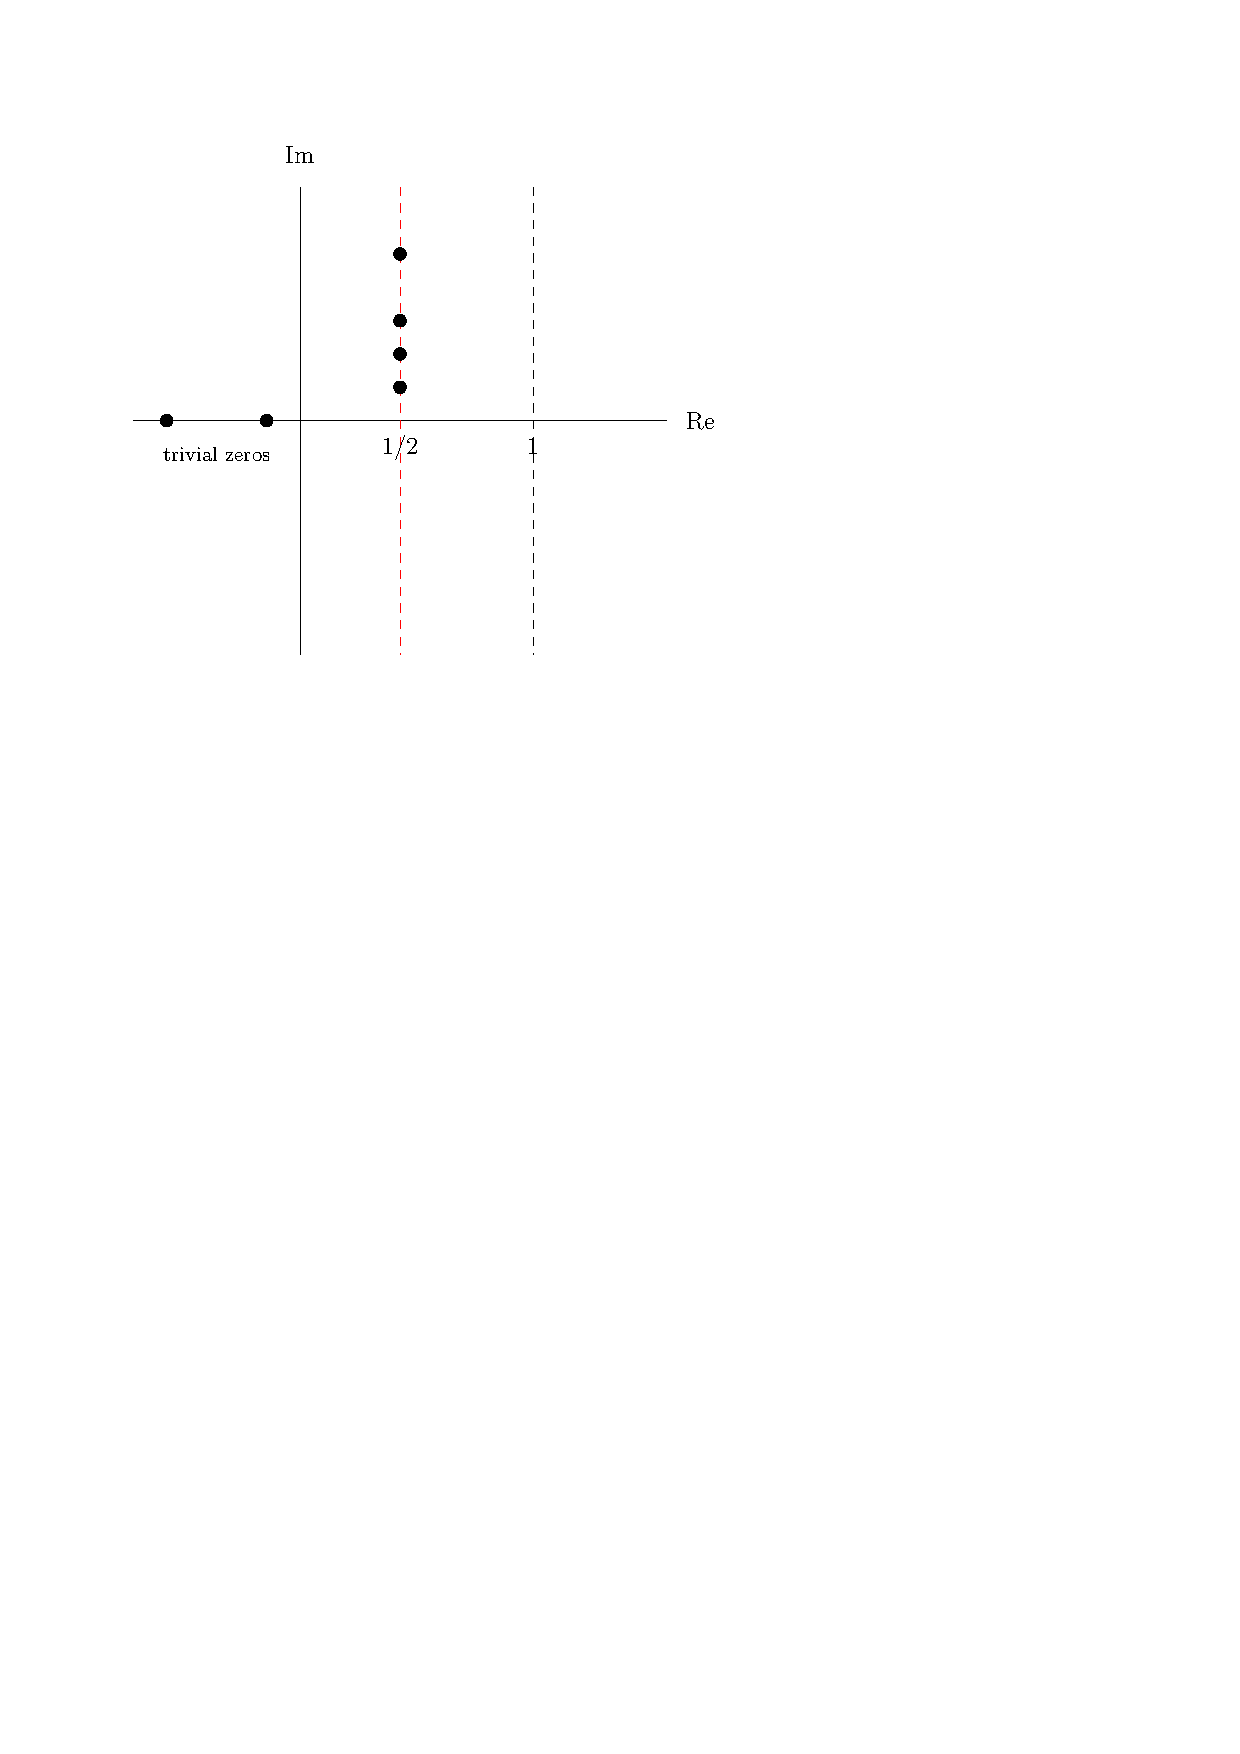
\includegraphics[width=.5\linewidth]{figures/riemann-hypothesis.pdf} 
    \caption{The non-trivial zeros of $\zeta(z)$ on a complex plane.}
    \label{fig:riemann-hypothesis}
\end{figure}

\section{Sum of Two Squares}

Recall that $a \equiv b \mod c$ if and only if $c \divides (a-b)$. 

If $p \equiv 1 \mod 4$, we will show that $p = a^2 + b^2$ for some integers $a$ and $b$. Such pair of $a,b$ where $a,b \in \Z$ is called a \textit{\textbf{lattice point}}.

\begin{theorem}[Fermat's theorem on sum of two squares]
    An odd prime $p$ can be expressed as $p = x^2 + y^2$ with integers $x$ and $y$ if and only if $p \equiv 1 \mod 4$.
\end{theorem}

Let $r_2(n)$ denote the number of representations of $n$ as a sum of two squares. We would like to study the behavior of $\sum_{n \leq x} r_2(n)$.

We start with \textbf{Gauss's attempt} in trying to bound $\sum_{n \leq x} r_2(n)$. As we can see, each lattice point can be represented as the coordinate $(m,n)$ of a point on a plane. If we draw a circle with radius $r$, then all lattice points within the circle have the property
$$
m^2 + n^2 \leq r^2
$$
Then, the problem of bounding $\sum_{n\leq x}r_2(n)$ for some $x$ is the same as finding the number of lattice points within the circle centered at $(0,0)$ with radius $\sqrt{x}$. Because of this, the problem is also known as \textit{\textbf{Gauss circle problem}}.

\begin{figure}[htbp]
    \centering
    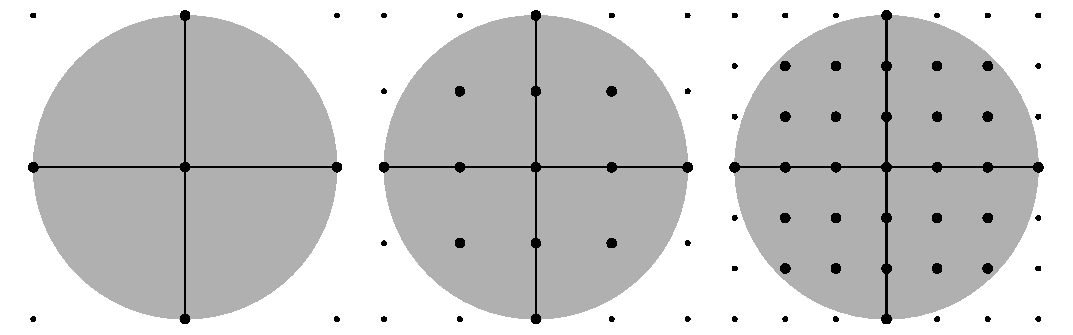
\includegraphics[width=0.5\linewidth]{figures/GausssCircleProblem.pdf}
    \caption{Gauss's circle problem}
    \label{fig:gauss-circle-prob}
\end{figure}

\begin{theorem}[Gauss's solution]
    $$
    \sum_{n \leq x} r_2(n) = \pi x + O(\sqrt{x}) = \pi x + \underbrace{E(x)}_{\text{error term}}
    $$
    So, $E(x) \in O(x^{1/2})$.
\end{theorem}

\begin{proof}
    We associate each representation of a number as two squares with a square on the plane, enclosed within the circle of radius $\sqrt{x}$.

    Then, the number of such lattice points is bounded above by the area of the larger circle and bounded below by the smaller circle.
    $$
    \pi(\sqrt{x} - 1)^2 \leq \sum_{n \leq x}r_2(n) \leq \pi(\sqrt{x} + 1)^2
    $$
    \begin{figure}[htbp]
        \centering
        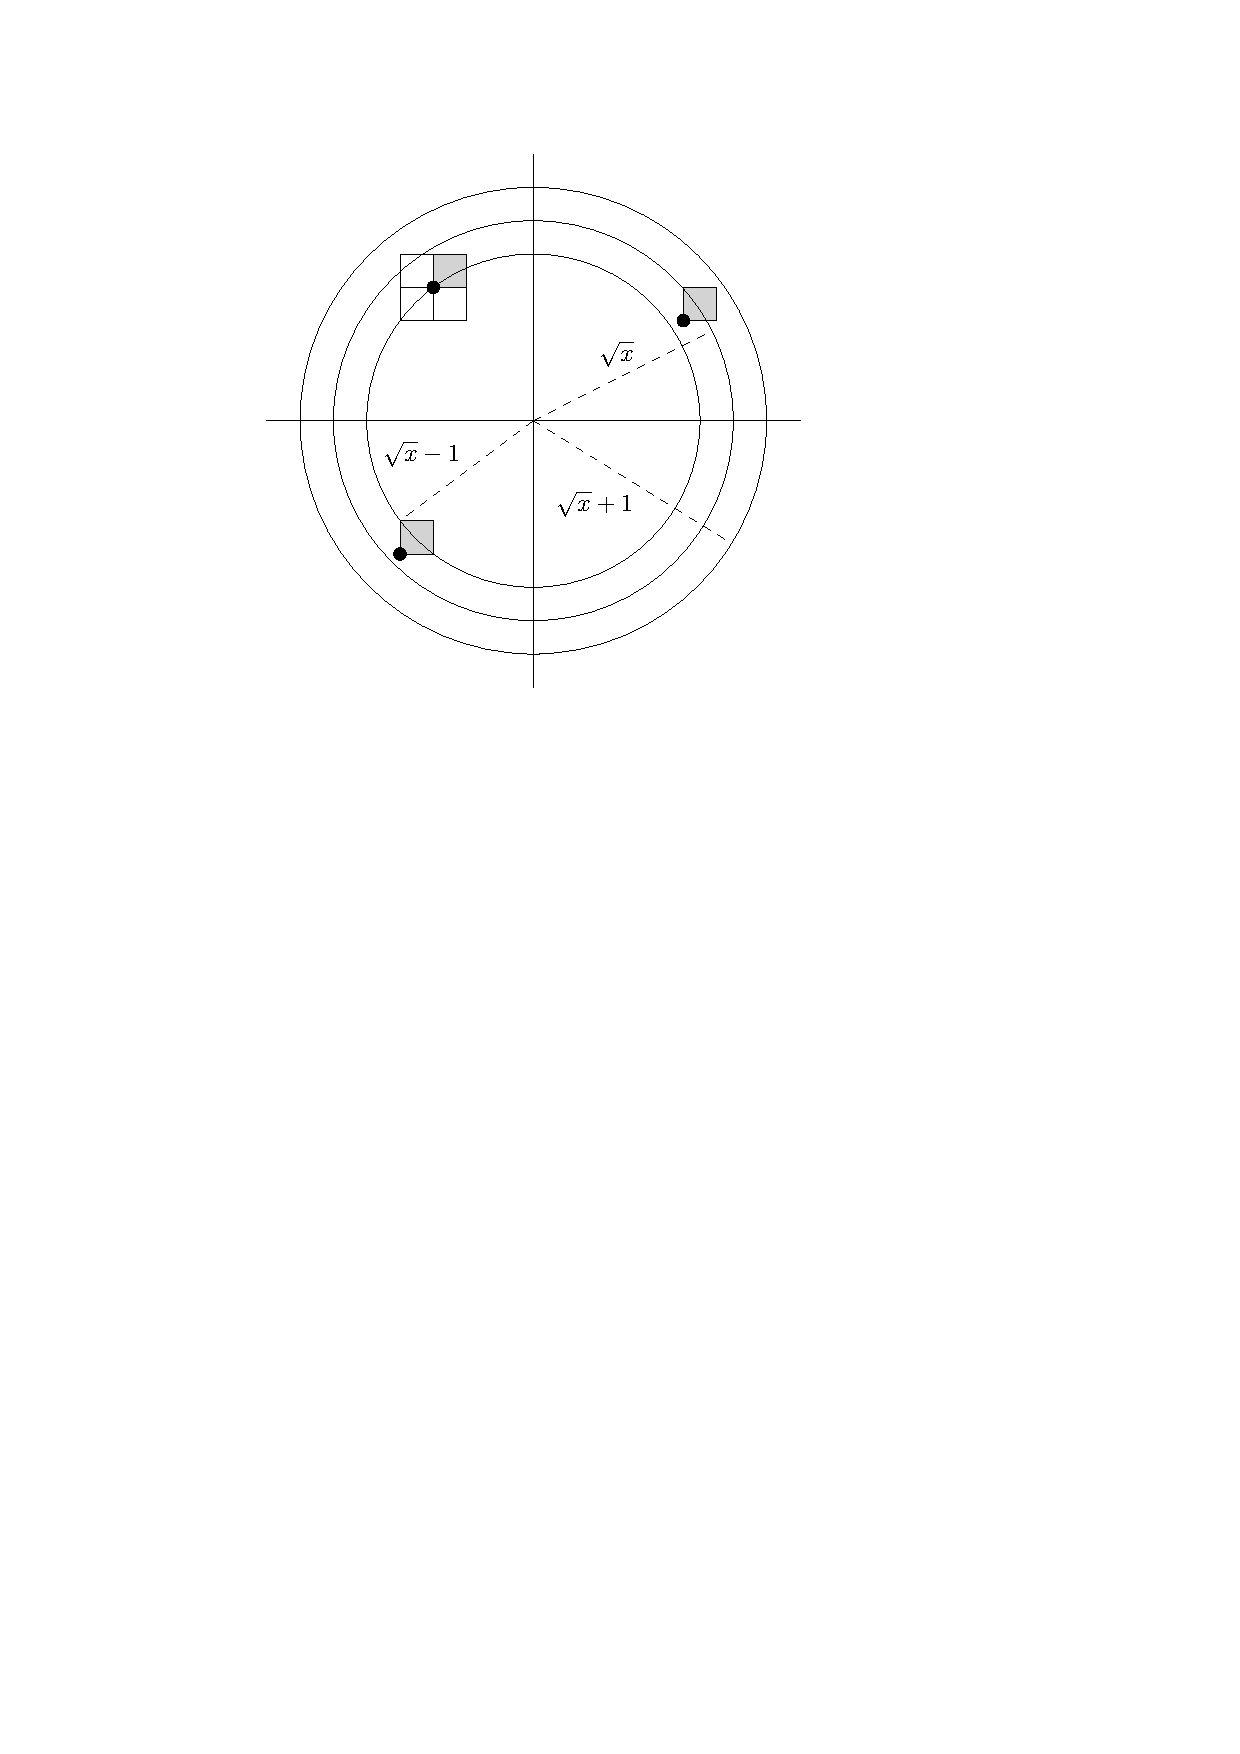
\includegraphics[width=.4\linewidth]{figures/gauss-circle-area.pdf}
        \caption{Using area to bound the number lattice points.}
        \label{fig:gauss-circle-area}
    \end{figure} 
    We can further rearrange this to get
    $$
    \pi(x - 2\sqrt{x+1}) \leq \sum_{n \leq x} r_2(n) \leq \pi(x + 2\sqrt{x} + 1)
    $$
    Then, $\sum_{n\leq x}r_2(n) = \pi x + O(\sqrt{x})$. 
\end{proof}

Over the years, there have been numerous improvements on bounding the error term.

\begin{theorem}[Sierpinski 1906]
    $$
    \sum_{n \leq x} r_2(n) = \pi x + O(x^{1/3})
    $$
\end{theorem}

\section{Integer Partition}

Next, we will consider the integer partition. A \textit{\textbf{partition}} of an integer $n \in \Z^+$ is one way of representing $n$ as a sum of \textbf{more than one} (possibly repeating) integers.

We define $P(n)$ to be the number of ways of writing $n \in \Z^+$ as a sum of positive integers (ways to partition $n$).

For example, $P(4) = 5$ because $4 = 3+1 = 2+2 = 2+1+1 = 1+1+1+1$. Note that $4$ itself does not count since we need at least 2 integers for it to be a valid partition.

\begin{conjecture}[Ramanujan's Conjecture on Integer Partition]
    $P(5n + 4) \equiv 0 \mod 5$, $P(7n + 5) \equiv 0 \mod 7$, $P(11n + 6) \equiv 0 \mod 11$.
\end{conjecture}

\part{Divisibility and Factorization}

\chapter{The Division Algorithm}
Recall that we say $a$ \textbf{divides} $b$, denoted by $a \divides b$, if there exists $c \in \Z$ such that $b = ac$.

\section{Propositions About Division}

Before we talk about the division algorithm, we first introduce some useful propositions about division.

\begin{proposition}
    $a \divides b$ and $b \divides c$ $\implies$ $a \divides c$. 
\end{proposition}

\begin{proof}
    The proof is straightforward from the definition of the division relation.

    Since $a \divides b$, $\exists c_1 \in \Z.\, b = c_1a$. Similarly, $\exists c_2 \in \Z.\, c = c_2 b$ since $b \divides c$. We can then rewrite $c$ as $c = c_2 b = c_1c_2a = (c_1c_2)a$. Since $c_1$ and $c_2$ are all integers, $c_1c_2$ is also an integer. Then, by definition, $a \divides c$.
\end{proof}

\begin{proposition}
    If $c \divides a$ and $c \divides b$, then $\forall m,n \in \Z.\, c \divides (ma+nb)$.
\end{proposition}

\begin{proof}
    Again, this is immediate from the definition and basic arithmetics.

    Since $c \divides a$, $\exists c_1 \in \Z.\, a = c_1c$. Since $c \divides b$, $\exists c_2 \in \Z.\, b = c_2 c$.

    Let $m,n \in \Z$ be arbitrary. Then, $ma + mb = mc_1c+nc_2c = c(mc_1 + nc_2)$. By definition, $c \divides (ma + mb)$.
\end{proof}

\section{Floor and Ceiling}

\begin{definition}[Floor]
    The floor of $x$, denoted $\floor{x}$, is the greatest integer less than or equal to $x$.
\end{definition}

Similarly, we define the ceiling as follows

\begin{definition}[Ceiling]
    The ceiling of $x$, denoted $\ceil{x}$, is the smallest integer greater than or equal to $x$.
\end{definition}

\begin{remark}
    In his lecture notes, Professor Berndt used $[\cdot]$ for floor. I decided to use the more standard notation in my notes to avoid confusion.
\end{remark}

\begin{lemma} \label{lem:div-algo-lem1}
    For $x \in \R$, $x-1 < \floor{x} \leq x$.
\end{lemma}

\begin{proof}
    By contradiction. Suppose not, then there exists some $x \in \R$ such that $x-1 \geq \floor{x}$. Take such $x$ and add 1 to both sides of the inequality, yielding $x \geq \floor{x} + 1$. But by definition, $\floor{x}$ is the greatest integer less than or equal to $x$. The fact that $\floor{x}+1$, which is strictly greater than $\floor{x}$, is also less than or equal to $x$ contradicts the definition of floor. Therefore, the original lemma holds. 
\end{proof}

\section{The Division Algorithm}

The \textbf{division algorithm} is also known as the \textbf{quotient remainder theorem}. The statement is as follows.

\begin{theorem}[The Division Algorithm]
    Let $a,b \in \Z$ such that $b > 0$. Then, there exists unique $q,r \in \Z$ such that $a = bq + r$ and $0 \leq r < b$.    
\end{theorem}

\begin{proof}
    We divide the proof into two parts: existence and uniqueness. We first prove \textbf{existence} by construction.

    Take $q = \floor{a/b}$ and $r = a - b \floor{a/b}$. Then, we have
    $$
    a = b \left\lfloor \frac{a}{b} \right\rfloor + r
    $$
    This proves that $a = bq + r$. Next, we show that $0 \leq r < b$. By Lemma \ref{lem:div-algo-lem1}, 
    $$
    \frac{a}{b} - 1 < \left\lfloor \frac{a}{b} \right\rfloor \leq \frac{a}{b}
    $$
    Since $b > 0$, we can multiply both sides by $b$, yielding
    $$
    a - b < \left\lfloor \frac{a}{b} \right\rfloor b \leq a
    $$
    Mutiply by -1 and reversing the signs, and then add $a$ to both sides
    $$
    \begin{aligned}
        b - a &> - \left\lfloor \frac{a}{b} \right\rfloor b &\geq -a \\
        b &> - \left\lfloor \frac{a}{b} \right\rfloor b + a &\geq 0
    \end{aligned}
    $$
    Since $r = a - b \floor{a/b}$, by substitution, $b > r \geq 0$. This proves the existence of such $q,r$.

    Next, we prove the \textbf{uniqueness} of such $q$ and $r$ by contradiction. Suppose for contradiction that there exists some $q' \neq q$ and $r' \neq r$ such that $a = bq' + r'$ and $0 \leq r' < b$. Then,
    $$
    a - a = 0 = b(q - q') + (r - r')
    $$
    $|r - r'| < b$ because both $r < b$ and $r' < b$. WLOG, suppose $r' > r$. Then, $r' - r = b(q' - q)$ by rearranging the previous inequality. This implies that $r' - r$ is a multiple of $b$. But since $r' - r$ is strictly less than $b$,
    $$
    0 \leq r' - r < b
    $$
    $r'-r$ must be 0. This contradicts the assumption that $r \neq r'$. Similarly, $q = q'$ since $r = r'$, which is also a contradiction.
\end{proof}

\chapter{Primes}
\section{Elementary Properties of Primes}

Recall that a natural number \textbf{greater than 1} is \textit{\textbf{prime}} if it has no factors other than 1 and itself. A natrual number greater than 1 is \textit{\textbf{composite}} if it is not prime.

We begin by introducing some elementary facts about prime numbers.

\begin{lemma} \label{lem:prime-divisor}
    Every integer greater than 1 has a prime divisor.
\end{lemma}

\begin{proof}
    By (strong) induction on $n$.

    \textbf{Base case}: $n = 2$. The lemma clearly holds because $2$ is a prime.

    \textbf{Inductive step}: Let $n \geq 2$ be an arbitrary integer. Suppose that the lemma is true for all integers $2 \leq n' < n$. If $n$ is prime, we are done. So assume $n$ is not prime. Then, by definition, $n$ is composite and can be expressed as $n = ab$ for some $a,b < n$. By induction hypothesis, $a$ and $b$ both have at least one prime divisors. Hence, $n$ also have a prime divisors.
\end{proof}

\begin{theorem}[Infinitude of Primes]
   There exists infinitely many primes. 
\end{theorem}

\begin{proof}
    By contradiction. Suppose there exist only finitely many primes $p_1,\ldots,p_n$.

    Let $N = p_1p_2\ldots p_n + 1$. By Lemma \ref{lem:prime-divisor}, $N$ has at least one prime divisor and since $\{p_1,\ldots,p_n\}$ are all the primes by assumption, there must exists some $i$ such that $p_i \divides N$. Since $p_i \in \{p_1,\ldots,p_n\}$, we have that $p_i \divides p_1\ldots p_n$ trivially. Further, $p_i \divides N$, so $p_i \divides N - p_1\ldots p_n$. This implies that $p_i \divides 1$. But no prime can divide 1. This is a contradiction.
\end{proof}

\begin{proposition}
    If $n$ is composite, then there exists at least one prime $p \leq \sqrt{n}$ dividing $n$.
\end{proposition}

\begin{proof}
    By contradiction. Let $n$ be an arbitrary composite number. By Lemma \ref{lem:prime-divisor}, we know that  has at least one prime divisor $p_j$. Suppose for contradiction that all such $p_j$ are $p_j > \sqrt{n}$.

    $n$ is composite, so we assume that it has $m$ divisors of $n$ where $m \geq 2$. Then,
    $$
    n > \underbrace{\sqrt{n} \sqrt{n} \cdots \sqrt{n}}_{m} = n^{m/2} \geq n
    $$
    This implies $n > n$, which is a contradiction.
\end{proof}

\section{Finding Primes}

Algorithm known as the Sieve\footnote{strainer, colanders, used for filtering; this name is likely due to the fact that the algorithm ``filters out'' the non-primes.} of Eratosthenes.

To find all primes $\leq x$, we list all integers up to $x$. Strike out every integer $\leq \sqrt{x}$ that is a multiple of primes $\leq \sqrt{x}$. In the end, whatever remains are primes.

\begin{example}[Finding primes $\leq 28$]
    List all numbers:

    2 3 4 5 6 7 8 9 10 11 12 13 14 15 16 17 18 19 20 21 22 23 24 25 26 27 28

    2 is prime, so we circle it. Then, we strike out all numbers that is a multiple of 2.

    \boxed{2} 3 \cancel{4} 5 \cancel{6} 7 \cancel{8} 9 \cancel{10} 11 \cancel{12} 13 \cancel{14} 15 \cancel{16} 17 \cancel{18} 19 \cancel{20} 21 \cancel{22} 23 \cancel{24} 25 \cancel{26} 27 \cancel{28}

    The next number, 3, is not struck out, so 3 is prime. We circle 3 and cross out all multiples of 3.

    \boxed{2} \boxed{3} \cancel{4} 5 \cancel{6} 7 \cancel{8} \cancel{9} \cancel{10} 11 \cancel{12} 13 \cancel{14} \cancel{15} \cancel{16} 17 \cancel{18} 19 \cancel{20} \cancel{21} \cancel{22} 23 \cancel{24} 25 \cancel{26} \cancel{27} \cancel{28}

    The next number, 5, is not struck out, so 5 is prime. We circle 5 and cross out all multiples of 5 that are not yet struck out.

    \boxed{2} \boxed{3} \cancel{4} \boxed{5} \cancel{6} 7 \cancel{8} \cancel{9} \cancel{10} 11 \cancel{12} 13 \cancel{14} \cancel{15} \cancel{16} 17 \cancel{18} 19 \cancel{20} \cancel{21} \cancel{22} 23 \cancel{24} \cancel{25} \cancel{26} \cancel{27} \cancel{28}

    Since $4 < \sqrt{28} < 5$, we can stop here and box all the remaining numbers. They are primes because they are not struck out.

    \boxed{2} \boxed{3} \cancel{4} \boxed{5} \cancel{6} \boxed{7} \cancel{8} \cancel{9} \cancel{10} \boxed{11} \cancel{12} \boxed{13} \cancel{14} \cancel{15} \cancel{16} \boxed{17} \cancel{18} 19 \cancel{20} \cancel{21} \cancel{22} \boxed{23} \cancel{24} \cancel{25} \cancel{26} \cancel{27} \cancel{28}
\end{example}

To test if a number $n$ is prime, we test all primes $p \leq \sqrt{n}$. If none divides $n$, then $n$ is prime. There are more efficient algorithms for primality testing. More recently, the AKS primality testing algorithm was shown to be able to run in polynomial time.

\section{Consecutive Composites}

\begin{proposition}
    For every $n \in \Z^+$, there exists $n$ consecutive composite numbers.
\end{proposition}

\begin{proof}
    By construction.

    $(n+1)! + 2$, $(n+1)! + 3$, $\ldots$, $(n+1)! + (n+1)$ are all composite.
\end{proof}

Note that this construction may not give the smallest $n$ consecutive composite numbers.

\section{Famous Conjectures About Primes}
\subsection{Goldbach's Conjecture}

\begin{conjecture}[Goldbach]
    Every even integer is a sum of two primes.
\end{conjecture}

\subsection{Mersenne Prime}

\begin{definition}
    Suppose $p$ is prime. If $2^p - 1$ is also a prime, we say that $p$ is a Mersenne prime.
\end{definition}

\begin{conjecture}[Infinitude of Mersenne Primes]
    There exist infinitely many Mersenne primes.
\end{conjecture}

As of October 2021, there are 51 known Mersenne primes. The largest known Mersenne prime is $2^{82,589,933} - 1$. Both the Mersenne prime problem and the Goldbach's conjecture are unsolved problems in number theory.

\section{Distribution of Primes}

Recall that from calculus, we know that
$
\sum_{n=1}^{\infty} \frac{1}{n} = \infty
$
but
$
\sum_{n=1}^{\infty} \frac{1}{n^2} = \frac{\pi^2}{6}.
$
Now, one might be interested in knowing how the series
$$
\sum_{\text{$p$ prime}} \frac{1}{p}
$$
behaves.

\begin{theorem}
    For every $y \geq 2$,
    $$
    \sum_{\substack{p \leq y \\ \text{$p$ prime}}} \frac{1}{p} \geq \log \log y - 1
    $$
\end{theorem}

\begin{proof}
    Let $\mathcal{N}$ be the subset of $\Z^+$ whose prime factorizations contain only primes $\leq y$. Consider $\sum_{n=1}^{\floor{y}} 1/n$, which is an upper bound on the sum that we are interested in.
    \begin{equation}
    \sum_{n=1}^{\floor{y}} \frac{1}{n} \geq \int_{1}^{\floor{y} + 1} \frac{dx}{x} = \log (\floor{y}+1) \geq \log (y)
    \end{equation}
    Now, consider the product of the geometric series over all primes $p \leq y$.
    \begin{equation}
        \prod_{\substack{p \leq y \\ \text{$p$ prime}}} \left( \sum_{i=0}^\infty \frac{1}{p^i} \right) = \prod_{\substack{p \leq y \\ \text{$p$ prime}}} \frac{1}{1 - 1/p} = \sum_{n \in \mathcal{N}} \frac{1}{n} \geq \sum_{n=1}^{\floor{y}} \frac{1}{n} \geq \int_{1}^{\floor{y} + 1} \frac{dx}{x} \geq \log y
    \end{equation}
    \textit{Claim}. For $0 \leq v \leq \frac{1}{2}$, $e^{v+v^2} \geq \frac{1}{1-v}$. Let $v = 1/p \leq 1/2$.

    Then, from the claim,
    \begin{equation}
    \prod_{\substack{p \leq y \\ \text{$p$ prime}}} e^{\frac{1}{p} + \frac{1}{p^2}} \geq \prod_{\substack{p \leq y \\ \text{$p$ prime}}} \frac{1}{1-1/p} \geq \log y
    \end{equation}
    Take the logarithm of both sides,
    \begin{equation}
        \log \prod_{\substack{p \leq y \\ \text{$p$ prime}}} e^{\frac{1}{p} + \frac{1}{p^2}} \leq \sum_{\substack{p \leq y \\ \text{$p$ prime}}} \log e^{\frac{1}{p} + \frac{1}{p^2}} = \sum_{\substack{p \leq y \\ \text{$p$ prime}}} \left( \frac{1}{p} + \frac{1}{p^2} \right) \geq \log \log y 
    \end{equation}
    Further, we observe that
    \begin{equation}
        \sum_{\substack{p \leq y \\ \text{$p$ prime}}} \frac{1}{p^2} \leq \sum_{n=2}^{\infty} \frac{1}{n^2} = \frac{\pi^2}{6} < 1
    \end{equation}
    So it follows that
    \begin{equation}
        \sum_{\substack{p \leq y \\ \text{$p$ prime}}} \frac{1}{p} > \log \log y - \sum_{\substack{p \leq y \\ \text{$p$ prime}}} \frac{1}{p^2} > \log \log y - 1
    \end{equation}
\end{proof}

We must also prove the claim we have used in the proof of the theorem.

\begin{lemma}
    For $0 \leq v \leq 1/2$,
    $$
    e^{v+v^2} \geq \frac{1}{1-v}
    $$
\end{lemma}
\begin{proof}
    Let $f(v) = (1-v) e^{v + v^2}$. $f(0)= 1$. We see that the first derivative is non-negative and thus $f$ is non-decreasing on $[0,\frac{1}{2}]$.
    $$
    f'(v) = -e^{v+v^2} + (1-v)(1+2v)e^{v+v^2} = v(1-2v)e^{v+v^2}.
    $$
    Then, since $f(v) = (1-v) e^{v+v^2}$ is non-decreasing on $[0,1/2]$, we have
    $$
    f(v) = (1-v) e^{v+v^2} \geq f(0) = 1 \qquad \forall v \in [0,1/2]
    $$
    This implies that $e^{v+v^2} \geq \frac{1}{1-v}$ for $0 \leq v \leq 1/2$.
\end{proof}


\chapter{Greatest Common Divisor and the Euclidean Algorithm}
\section{GCD}

GCD stands for greatest common divisor, as defined here.

\begin{definition}[Greatest Common Divisor]
    Let $a,b \in \Z$. The \textit{\textbf{greatest common divisor}} of $a$ and $b$ is the largest of all common divisors of $a$ and $b$. The notation for the GCD of $a$ and $b$ is $(a,b)$ or $\gcd(a,b)$.
\end{definition}

\begin{proposition}
    $\gcd(\frac{a}{d}, \frac{b}{d}) = 1 \iff (a,b) = d$ 
\end{proposition}

\begin{proof}
    \hfill

    ($\impliedby$): Suppose $\gcd(a,b) = d$ and $\gcd(\frac{a}{d}, \frac{b}{d}) = d'$. We want to show that $d' = 1$. By definition,
    $$
    d' \divides \frac{a}{d} \implies \frac{a}{d} = c_1 d' \implies a = c_1d'd
    $$
    and
    $$
    d' \divides \frac{b}{d} \implies \frac{b}{d} = c_2 d' \implies b = c_2d'd
    $$
    Thus, $d'd$ is also a common divisor of $a$ and $b$. Since $d$ is the \textbf{greatest} common divisor, $d' = 1$. Otherwise, it would contradict the maximality of $d$.

    ($\implies$): Suppose $\gcd(\frac{a}{d},\frac{b}{d}) = 1$ and $\gcd(a,b) = d'$. Then,
    $$
    d' \divides a \implies a = d' c_1 \implies \frac{a}{d} = \frac{d}{d'} c_1
    $$
    and
    $$
    d' \divides b \implies b = d' c_2 \implies \frac{b}{d} = \frac{d}{d'} c_2
    $$
    Thus, $d'/d$ is a common divisor of $\frac{a}{d}$ and $\frac{b}{d}$. Since $\gcd(\frac{a}{d}, \frac{b}{d}) = 1$, $d' = d$. So, $\gcd(a,b) = d$.
\end{proof}

\begin{proposition} \label{prop:gcd-linear-combination}
    Let $a,b \in \Z$ such that at least one of the two is not 0. Then,
    $$
    \gcd(a,b) = \min\{ma+nb > 0 \mid m,n \in \Z\} > 0
    $$
\end{proposition}

\begin{proof}
    We first show that $\{ma+nb > 0 \mid m,n \in \Z\}$ is not empty. This is trivial because we can arbitrary choose some $m,n$ such that $ma+nb > 0$.

    By the Well Ordering Principle, $\{ma+nb > 0 \mid m,n \in \Z\}$ has a minimum. Let $d = m'a + n'b$ be such minimal element.

    To prove the proposition, it suffices to show that $d$ is a common divisor of $a$ and $b$ and that $d$ is the greatest common divisor.

    \textit{Claim}: $d \divides a$ and $d \divides b$. WLOG, $b \geq a > 0$. By the division algorithm, $a = dq + r$ where $0 \leq r < d$. Rearrange this and we get
    $$
    r = a - dq = a - (m'a + n'b) q = (1 - m'q) a + n'q b
    $$
    Note that unless $r = 0$, $r$ would be a smaller linear combination of $a$ and $b$, contradicting the minimality of $d = m'a + n'q$. Therefore, $r = 0$. This implies $a = dq$ so $d \divides a$. The same argument also shows that $d \divides b$.

    \textit{Claim}: $d$ is the greatest common divisor of $a$ and $b$. Let $c$ be an arbitrary common divisor of $a$ and $b$. We want to show that $d \geq c$ for all possible choice of $c$. Since $c$ is a common divisor of $a$ and $b$, it is also a common divisor of $(m'a+n'b)$. Hence, $c \divides (m'a + n'b)$ so $c \divides d$. This implies that $c \leq d$.

    Combining the two claims proves that $d$ is the greatest common divisor.
\end{proof}

\section{Euclidean Algorithm}

Proposition \ref{prop:gcd-linear-combination} gives us a way to find the greatest common divisor between two numbers. But it is not easy to compute. The Euclidean algorithm is an easier and more commonly used algorithm for finding the GCD.

\begin{lemma} \label{lem:eucliean-algo-lemma}
    Let $a,b \in \Z^+$ such that $a \geq b$. Let $a = bq + r$ for $q,r \in \Z$. Then, $\gcd(a,b) = \gcd(b,r)$.
\end{lemma}

\begin{proof}
    To prove the lemma, it suffices to prove that for $a = bq + r$, $\gcd(a,b) = c$ if and only if $\gcd(b,r)= c$.

    Let $c$ be such that $c \divides a$ and $c \divides b$. Then, $c \divides r$ because $r$ is a linear combination of $a$ and $b$.

    Let $c \divides b$ and $c \divides r$. Then, $c \divides a$ because $a$ is a linear combnation of $b$ and $r$. Putting the two parts together, we have $c = \gcd(b,r) = \gcd(a,b)$.
\end{proof}

Now we are ready to state the Eucliean algorithm.

\begin{theorem}[Euclidean Algorithm]
    Let $a,b \in \Z^+$ with $a \geq b > 0$. By the division algorithm, 
    $$
    a = bq_1 + r_1
    $$
    for some $q_1,r_1 \in \Z$ such that $0 \leq r_1 < b$. 
    
    If $r_1 > 0$, we apply the division algorithm by letting
    $$
    b = r_1 q_2 + r_2
    $$
    for some $q_2,r_2 \in \Z$ such that $0 \leq r_2 < r_1$.

    If $r_2 > 0$, we apply the division algorithm again by letting
    $$
    r_1 = r_2q_3 + r_3
    $$
    for some $q_3,r_3 \in \Z$ such that $0 \leq r_3 < r_2$.

    Repeat until $r_n = 0$ for some $n$. If $n > 1$, then $\gcd(a,b) = r_{n-1}$. If $n=1$, $\gcd(a,b) = b$.
\end{theorem}

\begin{proof}
    We first observe that the algorithm terminates after a finite amount of iterations since $r_1 > r_2 > \cdots > r_n = 0$ is a strictly decreasing sequence of positive integers.

    If $n = 1$, $r_1 = 0$. In this case, $a = bq_1$ for some $q_1$ and $b \divides a$. It follows that $\gcd(a,b) = b = \gcd(b,0)$.

    Otherwise,
    $$
    \gcd(a,b) = \gcd(b,r_1) = \gcd(r_1,r_2) = \cdots = \gcd(r_{n-1}, r_n) = \gcd(r_{n},0)
    $$
    by repeated application of Lemma \ref{lem:eucliean-algo-lemma}.
\end{proof}

\section{Least Common Multiple}

\begin{definition}[Least Common Multiple]
    Let $a,b \neq 0$. The \textit{\textbf{least common multiple}} of $a$ and $b$, denoted by $[a,b]$ or $\lcm(a,b)$, is the least $m > 0$ such that $a \divides m$ and $b \divides m$.
\end{definition}

\begin{example}
    What is $\lcm(2^3 3^2 7^5,\, 2 \cdot 3^5 7 \cdot 11^2)$? \\
    We take the least common multiple of each factor, so we have $2^3 3^5 7^5 11^2$ 
\end{example}

If $\gcd(a,b) = 1$, $\lcm(a,b) = ab$. In general, we have the following theorem

\begin{theorem}
    $
    \gcd(a,b) \cdot \lcm(a,b) = ab
    $
\end{theorem}

\begin{proof}
    Assume $a,b > 1$. If either $a$ or $b$ is equal to 1, then the proof is trivial. Let
    $$
    a = p_1^{a_1} p_2^{a_2} \cdots p_n^{a_n} \qquad b = p_1^{b_1} p_2^{b_2} \cdots p_n^{b_n}
    $$
    so that $p_1,\ldots,p_n$ are the primes in common to $a$ and $b$. Since $\gcd(a,b)$ is the greatest common \textbf{divisor},
    $$
    \gcd(a,b) = p_1^{\min(a_1,b_1)} p_2^{\min(a_2,b_2)} \cdots p_n^{\min(a_n,b_n)}
    $$
    Also,
    $$
    \lcm(a,b) = p_1^{\max(a_1,b_1)} p_2^{\max(a_2,b_2)} \cdots p_n^{\max(a_n,b_n)}
    $$
    Multiply the two together and we get
    $$
    \gcd(a,b) \cdot \lcm(a,b) = p_1^{a_1+b_1} \cdots p_n^{a_n + b_n} = (p_1^{a_1} \cdots p_n^{a_n}) \cdot (p_1^{b_1} \cdots p_n^{b_n}) = ab
    $$
\end{proof}

In practice, we can use theorem to find the least common multiple once we find the greatest common divisor using the Euclidean algorithm.


\chapter{Fundamental Theorem of Arithmetics}
\section{Fundamental Theorem of Arithmetic}

Now we introduce a few lemmas in preparation for the Fundamental Theorem of Arithmetic.

\begin{lemma} \label{lem:unique-factor-lem}
    Let $p$ be prime such that $p \divides ab$. Then, $p \divides a$ or $p \divides b$.
\end{lemma}

\begin{proof}
    Assume that $p \divides ab$. If $p \divides a$, then we are done, so assume that $p \notdivides a$. Then, $a$ and $p$ are coprime, so $\gcd(p,a) = 1$. There exists some $m,n \in \Z$ such that $ma + np = 1$ by Prop 4.2.

    $b = 1 \cdot b$ so $b = mab + npb$. By assumption, $p \divides ab$. Then, there exists $c \in \Z$ such that $ab = pc$. It follows that
    $$
    b = mpc + npb = p(mc+nb)
    $$
    which, by definition of divisiblity, $p \divides b$.
\end{proof}

\begin{corollary} \label{cor:fta-cor}
    Let $p$ be prime, $a_1,\ldots,a_n \in \Z$ for $n \geq 2$. If $p \divides a_1a_2\ldots a_n$, then $p \divides a_j$ for at least one $j \in \{1,2,\ldots,n\}$.
\end{corollary}

\begin{proof}
    By Lemma \ref{lem:unique-factor-lem}, $p \divides a_1\ldots a_{n-1}$ or $p \divides a_n$. Prove by induction on $n \geq 2$.
\end{proof}

\begin{theorem}[Fundamental Theorem of Arithmetic]
    Every integer $a > 1$ can be represented \textbf{uniquely} as a product of primes
    $$
    a = p_1^{a_1} p_2^{a_2} \cdots p_n^{a_n}
    $$
    where $p_i \neq p_j$ if $i \neq j$ for positive integers $a_i$.
\end{theorem}

Now, we are ready to prove the \textit{\textbf{Fundamental Theorem of Arithmetic}}. It states the factorizability of any positive integers so the theorem is sometimes called the unique factorization theorem.

\begin{proof}
    By contradiction.

    Assume that there exists some integer without a prime factorization. Take $c$ to be the smallest of such counterexamples. Then, $c$ must be composite (otherwise, $c$ itself would be a unique prime factorization of $c$). Then, $c = ab$ for some $a,b > 1$ and $a,b < c$. Since $c$ is the smallest counterexample, $a$ and $b$, which are smaller than $c$, can be represented as products of primes. Therefore, $c$ indeed has a prime factorization that is the product of the prime factorizations of $a$ and $b$. This is a contradiction, so $c$ \textbf{has a prime factorization}.

    It remains to be shown that the factorization of $c$ is unique. Suppose for contradiction that $c$ has two prime factorizations. That is
    $$
    c = p_1^{a_1} p_2^{a_2} \cdots p_m^{a_m} = q_1^{b_1} q_2^{b_2} \cdots q_n^{b_n}
    $$
    where $p_1 < p_{i+1}$ and $q_{j} < q_{j+1}$ for all $i \in \{1,\ldots,m-1\}$ and $j \in \{1,\ldots,n-1\}$.

    It suffices to show that $p_j = q_j$, $a_j = b_j$ for all $j$, $m = n$.
    
    Fix arbitrary $p_i$. By Corollary \ref{cor:fta-cor}, $p_i \divides q_j$ for some $j$. Since $p_i$ and $q_j$ are prime, it follows that $p_i = q_j$ because otherwise it would be a contradiction. Similarly, fix $q_j$, and by the same argument, $q_j \divides p_i$ for some $i$ so $p_i = q_j$. Thus, $p_j = q_j$ for all $j$. This also implies that $m = n$.

    Finally, we show that the exponents are also equal. Suppose for contradiction that there exists some $j$ such that $a_j \neq b_j$. Without loss of generality, assume $a_j < b_j$. Since
    $$
    p_j^{b_j} \divides c = p_1^{a_1} p_2^{a_2} \cdots p_n^{a_n}
    $$
    so $p_1^{a_1} p_2^{a_2} \cdots p_n^{a_n} = k p_j^{b_j}$ for some $k \in \Z$. It follows that by dividing both sides by $p_j^{a_j}$,
    $$
    p_1^{a_1} p_2^{a_2} \cdots p_{j-1}^{a_{j-1}} p_{j+1}^{a_{j+1}} \cdots p_n^{a_n} = k p_{j}^{b_j - a_j}
    $$
    Since $b_j - a_j > 0$, $p_j \divides p_1^{a_1} p_2^{a_2} \cdots p_{j-1}^{a_{j-1}} p_{j+1}^{a_{j+1}} \cdots p_n^{a_n}$. By Corollary \ref{cor:fta-cor}, $p_j \divides p_i$ for some $i \neq j$. But this is not possible because for all $i \in \{1\ldots n\} \setminus \{j\}$, $p_i$ is prime and $p_j$ is \textbf{not a factor} of $p_1^{a_1} p_2^{a_2} \cdots p_{j-1}^{a_{j-1}} p_{j+1}^{a_{j+1}} \cdots p_n^{a_n}$. Hence, $p_i \divides p_j$ and $p_i \neq p_j$, which is a contradiction because a prime cannot divide another prime.

    Therefore, the prime \textbf{factorization is unique}.
\end{proof}

\chapter{Dirichlet's Theorem}
\section{Arithmetic Progression and Dirichlet's Theorem}

Arithmetic progression is another name for the arithmetic sequence, a sequence of integers in which the difference between two consecutive numbers is constant. In general, the $n$th term in an arithmetic sequence/progression is given by
$$
a_n = a_1 + (n-1) d
$$
How many primes are there in an infinite arithmetic progression? The theorem of Dirichlet tells us that indeed there are infinitely many primes in an infinite arithmetic progression.

\begin{theorem}[Dirichlet's Theorem on Primes in Arithmetic Progression]
    If $\gcd(a,b)=1$ ($a$ and $b$ are \textbf{relatively prime}), then the set
    $$
    \{ an + b \mid n \in \Z,\, n \geq 0 \}
    $$
    has \textbf{infinitely} many primes.
\end{theorem}

The proof of Dirichlet's theorem is beyond the scope of this course but will be covered in a course on analytic number theory. We can, however, prove some special cases of Dirichlet's theorem.

\subsection{Special Cases of Dirichlet's Theorem}
\begin{lemma} \label{lem:dirichlet-special-case-lem}
    Let $a,b \in \Z^+$. Suppose $a,b \in \{4n+1 \mid n \in \Z,\, n \geq 0\}$. Then, $ab \in \{4n+1 \mid n \in \Z,\, n \geq 0\}$.
\end{lemma}

\begin{proof}
    Let $a = 4n_1 + 1$ and $b = 4n_2 + 1$. Then,
    $$
    ab = (4n_1 + 1) (4n_2 + 1) = 16n_1n_2 + 4(n_1+n_2) + 1
    $$
    which can be factored as $4(4n_1n_2 + n_1 + n_2) + 1$. Take $n = (4n_1n_2 + n_1 + n_2)$ which is clearly a non-negative integer. Then, $n = ab \in \{4n+1 \mid n \in \Z,\, n \geq 0\}$.
\end{proof}

Using this simple fact, we can show that there are infinitely many primes of the form $4n + 1$.

\begin{proposition}
    There exist infinitely many primes in $\{ 4n+3 \mid n \in \Z,\, n \geq 0\}$.
\end{proposition}

\begin{proof}
    By contradiction.

    Suppose for contradiction that there exist only finitely many primes in $\{ 4n+3 \mid n \in \Z,\, n \geq 0\}$. Say there exist only $r+1$ such primes. Clearly, $p_0 = 3$, and we have $p_0,p_1,\ldots,p_r$ from the set that are primes.

    Take $N = 4p_1p_2\cdots p_r + 3$. By the Fundamental Theorem of Arithmetic, $N$ has some prime divisor. We claim that $N$ has some prime divisor $q_j \in \{4n+3 \mid n\in \Z,\, n \geq 0\}$. Further, we claim that if not, all prime divisors of $N$ is of the form $4n + 1$. This is because we assumed that $q_j$ is a prime divisor and the prime numbers $\geq 3$ not of the form $4n + 3$ can be written as $4n + 1$ for some $n$. And if all prime divisors of $N$ are of the form $4n+1$, then $N$ must also be of the form $4n + 1$ by Lemma \ref{lem:dirichlet-special-case-lem}, which is not true. Then, $q_j$ is either 3 or one of $p_1,\ldots,p_r$.

    If $q_j = 3$, $q_j \divides 3$ and $q_j \divides N$. It follows that $q_j \divides (N-3)$ so $q_j \divides 4 p_1\cdots p_r$. This is a contradiction because $p_1,\ldots,p_r$ are primes not including 3. Hence, $q_j \neq 3$.

    If $q_j \in \{p_1,\ldots,p_r\}$, then $q_j \divides 4p_1\ldots p_r$. And by choice of $q_j$, $q_j \divides N$. It follows that $q_j \divides N - 4p_1\cdots p_r$. This implies $q_j \divides 3$, which is a contradiction as well becuase $3 \not\in \{p_1,\ldots,p_r\}$.

    In both cases, we have a contradiction so the assumption that there are finitely many primes of the form $4n + 3$ must be false.
\end{proof}

Note that this proof will not work for the general case of Dirichlet's theorem because Lemma \ref{lem:dirichlet-special-case-lem} does not hold in the general case.

Let's look another example of a similar special-case proof.

\begin{lemma}
    Let $a,b \in \Z^+$. Suppose $a,b \in \{3n+1 \mid n \in \Z,\, n \geq 0\}$. Then, $ab \in \{3n+1 \mid n \in \Z,\, n \geq 0\}$.
\end{lemma}

\begin{proof}
    Similar to the proof for Lemma \ref{lem:dirichlet-special-case-lem}.
\end{proof}

\begin{theorem}
    There exist infinitely many primes of the form $3n+2$ for $n \geq 0$.
\end{theorem}

\begin{proof}
    Suppose for contradiction that there exist only finitely many primes of the form $3n + 2$. Say there are $r+1$ such primes, namely, $2,p_1,\ldots,p_r$.

    Similar to the proof for the previous theorem, we let
    $$
    N = 3p_1\cdots p_r + 2
    $$
    We claim that there exsits a prime divisor of $N$ of the form $3n+2$. To see why this claim holds, assume that $N$ has no such divisors. Then, there are two possibilities for the prime divisors of $N$. First, we have $3 \divides N$. This is also not possible because $3 \notdivides 2$. This implies that $3n$ is not a prime divisor for $N$. The only remaining possiblity is that all prime divisors of $N$ are of the form $3n + 1$.

    However, by the previous lemma, we know that if all prime divisors of $N$ are of the form $3n + 1$, then $N$ itself must also be of the form $3n + 1$, which is not true. Hence, $N$ must have some prime divisor of the form $3n + 2$. Now, consider the following two cases regarding the prime divisor $q$ of $N$:

    Case 1: $q=2$. we have $2 \divides N$ and clearly $2 \divides 2$. It follows thata $2 \divides N - 2$, but this is a contradiction because $3p_1\cdots p_r$ does not contain 2 as a factor. Therefore, $q=2$ is not possible.

    Case 2: $q \in \{p_1,\ldots,p_r\}$. $q \divides N$ and $q \divides 3p_1\cdots p_r$. It follows that $q \divides 2$. But again, this is not possible becuase $q$ and $2$ are both primes.

    In both cases, we have a contradiction. This implies that $N$ itself is a prime that is not in $\{2,p_1,\ldots,p_r\}$. Hence, our initial assumption that there are finitely many primes of the form $3n + 2$ must be false, so the theorem holds.
\end{proof}

\part{Congruence}

\chapter{Congurence and Congruence Classes}
\section{Congruence}

\begin{definition}
    $a$ is congruent to $b$ modulo $m$ for $m \in \Z^+$ iff
    $$
    m \divides (a-b)
    $$
    and we write $a \equiv b \mod m$.
\end{definition}

For example, $3 \equiv 7 \mod 2$ because $3-7 = -4$ and $2 \divides -4$.

\begin{remark}
    Note that despite that congruence is denoted by $\equiv$, some properties of equality does not hold. Importantly, $ca \equiv cb \mod m$ DOES NOT imply $a \equiv b \mod m$. For a simple counterexample, consider $4 \equiv 6 \mod 2$ but $2 \not\equiv 3 \mod 2$.
\end{remark}

This tells us that we cannot just cancel common factors in a congruence relation. We established that in the general case, this will not work. For example, $6 \equiv 3 \mod 3$ but $2 \not\equiv 1 \mod 3$. However, there are cases where we can cancel factors in a congruence.

\begin{proposition} \label{prop:congruence-cancelation}
    $$
    ca \equiv cb \mod m \iff a \equiv b \mod \frac{m}{\gcd(c,m)}
    $$
\end{proposition}

For example, say we have $6 \equiv 3 \mod 3$. By Proposition \ref{prop:congruence-cancelation}, we have $2 \equiv 1 \mod \frac{3}{\gcd(3,3)}$ so $2 \equiv 1 \mod 1$. Now, we prove this proposition.

\begin{proof}

    ($\implies$):
    Assume that $ca \equiv cb \mod m$, which by definition, implies that $m \divides (ca-cb)$ and $m \divides c(a-b)$. By definition of divisibility, there exists some $d$ such that $c(a-b) = md$. Then, we can divide both sides by the greatest common divisor of $c$ and $m$, giving us
    $$
    \frac{c}{\gcd(c,m)} (a-b) = \frac{m}{\gcd(c,m)} d
    $$
    Further, since $\gcd(c,m)$ is the greatest common divisor, $\gcd\left(\frac{c}{\gcd(c,m)},\, \frac{m}{\gcd(c,m)} \right) = 1$. This implies
    $$
    \frac{m}{\gcd(c,m)} \divides (a-b)
    $$
    which by definition means $a \equiv b \mod \frac{m}{\gcd(c,m)}$.

    ($\impliedby$): Assume that $a \equiv b \mod \frac{m}{\gcd(c,m)}$. By definition, $\frac{m}{\gcd(c,m)} \divides (a-b)$. So there exists some $d$ such that
    $$
    a-b = \frac{m}{\gcd(c,m)}d \implies ca - cb = \frac{cm}{\gcd(c,m)} d = \frac{cd}{\gcd(c,m)} m
    $$
    This implies $m \divides (ca-cb)$ since $\frac{cd}{\gcd(c,m)}$ is an integer. Then by definition of congruence, $ca \equiv cb \mod m$.
\end{proof}

\subsection{Properties of Congruence Relation}

$$
\begin{aligned}
    &a \equiv a \mod m & \text{reflexive} \\
    &a \equiv b \mod m \iff b \equiv a \mod m & \text{symmetric} \\
    &a \equiv b \mod m \;\land\; b \equiv c \mod m \implies a \equiv c \mod m & \text{transitive}
\end{aligned}
$$

The reflexive and symmetric properties are obvious. We will provide a short proof for the transitive property.

\begin{proof}
    By definition of congruence, $a \equiv b \mod m$ means $m \divides (a-b)$. And $b \equiv c \mod m$ means $m \divides (b-c)$. It follows by property of divisibility that $m \divides (a-b+b-c)$. Then, $m \divides (a-c)$, which by definition means $a \equiv c \mod m$.
\end{proof}

Because of these three properties, we say that congruence defines an \textbf{equivalence relation}. Hence, equivalence relation of congruence divides integers into \textbf{equivalence classes}, known as the \textbf{congruence classes} or \textbf{residue classes}.

\section{Congruence Classes}

\begin{definition}[Congruence Classes]
    The congruence class of $a$ modulo $m$, denoted $[a]_m$, is the set of all integers that are congruent to $a$ modulo $m$
    $$
    \{ z \in \Z \mid m \divides (a-z) \}
    $$
\end{definition}

\begin{example}
    Let $m = 7$. Then,
    $$
    [0]_7 = \{\ldots,-14,-7,0,7,14,\ldots\}
    $$
    $$
    [1]_7 = \{\ldots,-13,-6,1,8,15,\ldots\}
    $$
    $$
    [2]_7 = \{\ldots,-12,-5,2,9,16,\ldots\}
    $$
    $$
    [3]_7 = \{\ldots,-11,-4,3,10,17,\ldots\}
    $$
\end{example}

\begin{definition}[Complete Residue System]
    A complete residue system modulo $m$ is a set $S$ of integers such that every $n \in \Z$ is congruent to one and only one member of $S$.
\end{definition}

\begin{example}
    $\{0,1,2,3,4,5,6\}$ is a complete residue system modulo $7$. \\ Although less obvious, $\{14,57,-12,1060,-24,-2,76\}$ is also a complete residue system modulo $7$.
\end{example}

\begin{proposition}
    $S = \{0,1,\ldots,m-1\}$ is a complete residue system modulo $m$.
\end{proposition}

\begin{proof}
    Let $a \in \Z$. Apply the division algorithm to $a$ with respect to $m$, so we have
    $$
    a = mq + r \qquad 0 \leq r \leq m-1
    $$
    By definition of divisibility, $m \divides (a-r)$, and by definition of congruence, $a \equiv r \mod m$. This shows that every integer is congruent to a member $r$ of $\{0,1,\ldots,m-1\}$.

    We also need to show that $a$ is congruent to only one member of $\{0,1,\ldots,m-1\}$. We proceed by contradiction. Assume $a \equiv r_1 \mod m$ and $a \equiv r_2 \mod m$ for some $r_1,r_2 \in \{0,1,\ldots,m-1\}$. By transitivity, $r_1 \equiv r_2 \mod m$, which by definition means $m \divides (r_1 - r_2)$. Since both $r_1$ and $r_2$ are between 0 and $m-1$, $0 \leq r_1-r_2 \leq m-1$. Then, $0 \leq r_1 - r_2 \leq m - 1$ and $m \divides (r_1-r_2)$ imply that $r_1-r_2 = 0$ because otherwise $m$ cannot divide any non-zero integers less than itself. This shows that $r_1 = r_2$ and thus uniqueness.
\end{proof}

\begin{proposition}
    Let $a,b,c,d \in \Z$. If $a \equiv b \mod m$ and $c \equiv d \mod m$, then
    \begin{equation} \label{eq:congruence-prop-1}
        a + c \equiv b + d \mod m
    \end{equation}
    \begin{equation} \label{eq:congruence-prop-2}
        ac \equiv bd \mod m
    \end{equation}
\end{proposition}

\begin{proof} of Equation (\ref{eq:congruence-prop-1})

    By definition of congruence, $m \divides (a-b)$ and $m \divides (c-d)$. By property of divisibility, $m \divides (a-b+c-d)$. This is equivalence to $m \divides [(a+c)-(b+d)]$, which by definition means $a+c \equiv b+d \mod m$.
\end{proof}

\begin{proof}
    of Equation (\ref{eq:congruence-prop-2})

    By definition, $m \divides (a-b)$ and $m \divides (c-d)$. Trivially, it follows that $m \divides c(a-b)$. Similarly, $m \divides b(c-d)$. By property of divisibility, $m \divides (ca-cb+bc-bd)$ so $m \divides (ac-bd)$. This by definition means $ac \equiv bd \mod m$.
\end{proof}

\section{Reduced Residue System}

Recall that we defined a \textit{\textbf{complete residue system}} as follows.

\begin{definition}[Complete Residue System]
    A \textbf{complete residue system} modulo $m$ is a set $S$ of integers such that every $n \in \Z$ is congruent to one and only one member of $S$.
\end{definition}

On the other hand, we define a reduced residue system as

\begin{definition}[Reduced Residue System]
    A \textbf{reduced residue system} modulo $m$ is a set of integers $r_1, \ldots, r_n$ such that if $\gcd(a,m) = 1$, then $a \equiv r_j \mod m$ for one and only one value of $j$.
\end{definition}

Stated slightly differently, a reduced residue system modulo $m$ is a set of integers $r_i$ such that $\gcd(r_i,m) = 1$ for all $i$, and $r_i \not\equiv r_j \mod m$ for all $j \neq i$. That is, each element in a reduced residue system is relatively prime to $m$ and no two elements of the set are congruent modulo $m$.

Note that the definition of a reduced residue system immediately implies that $n < m$. To see why, suppose $n = m$ and we have a complete residue system. Then, $m \equiv m \mod m$. WLOG, suppose $m = r_j$ for some $j$ (otherwise, we can choose $r_j$ to be some multiple of $m$). By definition, there's some $a$ such that $a \equiv m \mod m$ but this is impossible since $a$ and $m$ are relatively prime by definition of a reduced residue system. This implies that $m$ or any multiple of $m$ must not be an element in a reduced residue system.

Another way of looking at a reduced residue system is that we can take a complete residue system, remove certain numbers, and get back a reduced residue system. In particular, if we have a complete residue system modulo $m$, and we remove all $r_j$ such that $\gcd(r_j, m) \neq 1$, the resulting system is a reduced residue system. This should be clear from the definition of a reduced system.

Additionally, if $\gcd(a,m) = 1$ and $a \equiv r_j \mod m$ for some $a$, then $\gcd(r_j,m) = 1$. This essentially shows that our alternative definition is the same as the original definition.

\begin{proof}
    Suppose not. That is, there exists $a$ such that $\gcd(a,m) = 1$ and $m \divides (a-r_j)$ but $\gcd(r_j,m) \neq 1$. This implies there exists some $p$ such that $p \divides r_j$ and $p \divides m$. But we also have $a - r_j = md$ for some $d$ since $m \divides (a-r_j)$. This implies $p \divides a$. But by our assumption, $a$ and $m$ should be relatively prime, so this is a contradiction.
\end{proof}

\section{Euler's Phi Function}

The number of elements in a reduced residue system modulo $m$ for some fixed $m$ is \textbf{constant}. We call this number \textit{\textbf{Euler's phi function}} or \textit{\textbf{Euler's totient function}}. The Euler's phi function for $m$ is denoted by
$$
\varphi(m)
$$

\begin{theorem}
    Let $r_1,\ldots,r_n$ be a complete/reduced residue system modulo $m$. Let $\gcd(a,m)=1$. Then,
    $$
    \{ ar_1,\ldots, ar_n \}
    $$
    is still a complete/reduced residue system modulo $m$.
\end{theorem}

\begin{proof}
    Suppose for contradiction that $\{ar_1,\ldots,ar_n\}$ is not a complete/reduced residue system modulo $m$ for some $m$. Then, there must exitsts some $i$ and $j$ such that $ar_i \equiv ar_j \mod m$ (if no such $i,j$ exists, then $\{ar_1,\ldots,ar_n\}$ would indeed be complete/reduced). But since $\gcd(a,m) = 1$, $ar_i \equiv ar_j \mod m \iff r_i \equiv r_j \mod m$. This is a contradiction to the assumption that $\{r_1,\ldots,r_n\}$ is a complete/reduced residue system.
\end{proof}


\chapter{Linear Congruence}
\section{Linear Congruence}

We are all familiar with linear equations like
$$
ax + b = 0
$$
We are going to talk about a different kind of linear ``equation'' known as linear congruence. They are of the form
$$
ax \equiv b \mod m
$$
Let's consider some linear congruence. First, we look at $3x \equiv 1 \mod 6$. If we try everything from 0 to 5, it is easy to notice that this does not have a solution.

How about $2x \equiv 4 \mod 6$. We have one solution $\{2,8,14,\ldots,\}$ and another solution $\{5,11,17,\ldots\}$. In total, we have two solutions. Further, these two solution sets are incongruent because elements from one set is not congruent to those from the other set modulo $6$.

$2x \equiv 5 \mod 6$ does not have a solution. But $3x \equiv 1 \mod 5$ have the solution $\{2,7,12,\ldots,\}$.

The two examples that do not have a solution are $3x \equiv 1 \mod 6$ and $2x \equiv 5 \mod 6$. The ones that do have solutions are $2x \equiv 4 \mod 6$ and $3x \equiv 1 \mod 5$. From these examples, we make the observation that one thing in common among the linear congruences that do not have a solution is that the GCD of $a$ and $m$ does not divide $b$. In particular, we have that $\gcd(3,6) \notdivides 1$ and $\gcd(2,6) \notdivides 5$. On the other hand, $\gcd(2,6) \divides 4$ and $\gcd(3,5) \divides 1$.

We can generalize this into the following theorem:

\begin{theorem} \label{thm:lin-congruence-soln}
    Let $ax \equiv b \mod m$ be a linear congruence in one variable and let $d = \gcd(a,m)$. If $d \notdivides b$, then the linear congruence has no solution in $\Z$. If $d \divides b$, then the linear congruence has exactly $d$ incongruent solutions modulo $m$ in $\Z$.
\end{theorem}

The proof can be broken into two parts: 

(1) Showing that if $d \notdivides b$, then the linear congruence has no solution. This can be proved using the contrapositive of the original statement (namely, if the linear congruence has solution, then $d \divides b$); 

(2) Showing that if $d \divides b$, then the linear congruence has a solution, $x_0$. And given a solution $x_0$, we can construct infinitely many solutions of a given form and that among those infinitely many solutions, we have $d$ incongruent solutions. More specifically, it suffices to show the following:

\begin{addmargin}[1em]{0em}
    a. Show that a solution $x_0$ exists. \\
    b. Given a solution $x_0$, show that $ax \equiv b \mod m$ has infinitely many solutions in $\Z$ of a given form. \\
    c. Given a solution $x_0$, show that every solution has the form in (b). \\
    d. Show that there are $d$ incongruent solutions.
\end{addmargin}

\begin{proof}
    We begin the proof by proving \textbf{Part (1)} by its \textbf{contrapositive}.
    
    Assume that $ax \equiv b \mod m$ has a solution. By definition of congruence, $m \divides ax - b$. By definition of divisibility, $m \divides ax - b$ iff there exists some $y \in \Z$ such that $my = ax-b$. This, in turn, is true iff $ax - my = b$ has a solution. Since $d$ is the gcd of $a$ and $m$, $d \divides a$ and $d \divides m$. By Proposition 2.2, it follows that $d \divides ax - my$. Since $b = ax - my$ iff $ax \equiv b \mod m$ has a solution, $d \divides b$ if the original linear congruence has a solution.

    Now we proceed to prove \textbf{Part (2)a}. Assume $d \divides b$. Since $d$ is the \textbf{gcd} of $a$ and $m$, by \textbf{Proposition \ref{prop:gcd-linear-combination}}, there exists $r,s \in \Z$ such that
    $$
    d = ar + ms
    $$
    Further, $d \divides b$ implies $b = de$ for some $e \in \Z$. So, by substitution
    $$
    b = de = (ar + ms)e = a(re) + m(se)
    $$
    which clearly suggests a solution with $x = re$ and $y = -se$ that solves $ax - my = b$ (and thus solves $ax \equiv b \mod m$).

    For \textbf{Part (2)b}, let $x_0$ be an arbitrary solution for the linear congruence $ax \equiv b \mod m$. Let $n \in \Z$ and we consider
    $$
    x = x_0 + \left( \frac{m}{d} \right) n
    $$
    Since $d \divides m$, $\frac{m}{d}$ is an integer, so it follows that $x$ is also an integer. Furthermore, we observe that
    $$
    \begin{aligned}
        a\left( x_0 + \left( \frac{m}{d} \right) n \right) &= ax_0 + a\left( \frac{m}{d} \right) n \\
        &= ax_0 + \left( \frac{a}{d} \right) mn \\
        &\equiv ax_0 \mod m \\
        &\equiv b \mod m
    \end{aligned}
    $$
    Since for every solution $x$, $ax \equiv b \mod m$ but also $b \equiv a(x_0 + (\frac{m}{d})n) \mod m$, for all $n \in \Z$,
    $$
    x_0 + \left( \frac{m}{d} \right) n
    $$
    is also a solution to $ax \equiv b \mod m$. It follows that given any solution $x_0$ of $ax \equiv b \mod m$, there are infinitely many solutions of the form $x_0 + (m/d)n$ for $n \in \Z$.

    For \textbf{Part 2(c)}, let $x_0$ be a solution of $ax \equiv b \mod m$. Then, $ax_0 - my_0 = b$ for some $y_0 \in \Z$. Now, any other solution $x$ of $ax \equiv b \mod m$ implies the existence of $y \in \Z$ with $ax - my = b$, and we have
    $$
    (ax - my) - (ax_0 - my_0) = b - b = 0
    $$
    and
    $$
    a(x-x_0) = m(y-y_0)
    $$
    Dividing both sides by $d$, we have
    $$
    \left( \frac{a}{d} \right) (x-x_0) = \left( \frac{m}{d} \right) (y-y_0)
    $$
    Now $\frac{m}{d}\divides (\frac{a}{d}) (x-x_0)$. Since $\gcd(\frac{a}{d}, \frac{m}{d}) = 1$, we have $\frac{m}{d} \divides x-x_0$. Consequently, $x-x_0 = (\frac{m}{d}) n$ for some $n \in \Z$. Equivalently, $x = x_0 + (\frac{m}{d})n$ for some $n \in \Z$. Combining this result with 2(b), we hae shown that all solutions of $ax \equiv b \mod m$ are given precisely by $x_0 + (\frac{m}{d})n$ for $n \in \Z$.
    
    For \textbf{2(d)}, to determine how many incongruent solutions modulo $m$ exist among the solutions of the form $x_0 + (\frac{m}{d})n$ for $n \in \Z$, we establish a \textbf{necessary and sufficient condition} (chain of iff.) for the congruence modulo $m$ of two such solutions. Consider
    $$
    x_0 + \left( \frac{m}{d} \right) n_1 \equiv x_0 + \left( \frac{m}{d} \right) n_2 \mod m
    $$
    if and only if
    $$
    \left( \frac{m}{d} \right) n_1 \equiv \left( \frac{m}{d} \right) n_2 \mod m 
    $$
    if and only if
    $$
    m \divides \left( \frac{m}{d} \right) (n_1-n_2)
    $$
    if and only if
    $$
    d \divides n_1 - n_2
    $$
    if and only if
    $$
    n_1 \equiv n_2 \mod d
    $$
    Therefore, two solutions of the form $x_0 + (\frac{m}{d}) n$ are congruent modulo $m$ if and only if the $n$-values of these two solutions are congruent modulo $d$. Thus, a complete set of incongruent solutions modulo $m$ of $ax \equiv b \mod m$ can be obtained from an initial solution $x_0 + (\frac{m}{d})n$ by letting $n$ range over a complete residue system modulo $d$, that is $\{0,1,2,\ldots,d-1\}$.
\end{proof}

\begin{corollary} \label{cor:all-congruence-solutions}
    Let $ax \equiv b \mod m$ be a linear congruence in one variable and let $d = \gcd(a,m)$. If $d \divides b$, then there are $d$ incongruent solutions modulo $m$ given by
    $$
    x_0 + \left( \frac{m}{d} \right) n \qquad n = 0,1\ldots,d-1
    $$
    where $x_0$ is a particular solution of the congruence.
\end{corollary}

\section{Solving Linear Congruence}

It is perfectly acceptable to solve linear congruence by inspection (guess and check). However, for larger $m$, it might be too slow and tedious to solve the linear congruence simply by inspection. We now introduce a general procedure for solving linear congruence.

Recall that a linear congruence $ax \equiv b \mod m$ can always be expressed as $ax - my = b$ for some $y \in \Z$. We begin by considering an example:
$$
9x \equiv 21 \mod 30
$$
which is equivalent to $21 = 9x - 30y$. Since $\gcd(9,30) \divides 21$ so the linear congruence has solutions. We apply the Euclidean algorithm
$$
\begin{aligned}
    30 &= 3 \cdot 9 + \boxed{3} \\
    9 &= 3 \cdot 3 + 0
\end{aligned}
$$
So we know that $\gcd(9,30) = 3 = 1 \cdot 30 - 3 \cdot 9$ (recall that another way to look at gcd is as the minimum positive linear combination of the two numbers). Then, multiply both sides of the equation by 7 so that the LHS is equal to 21, and we have
$$
21 = (1 \cdot 7) 30 - (3 \cdot 7) \cdot 9
$$
Comparing this with the equation equivalent to our congruence equation, $21 = 9x - 30y$, we know that $x = -21$ and $y = -7$ is a solution. To get other olutions, we apply Corollary \ref{cor:all-congruence-solutions}, giving us $x = -21 + 10 = -11$, $x = -21 + 20 = -1$, $x = -21 + 30 = 9$, etc. Note that once we go above -1, all the other solutions may no longer be incongruent to the previous solutions.

\begin{example}[A harder example]
    Solve
    $$
    481x \equiv 627 \mod 703
    $$
\end{example}
Use the Euclidean algorithm to find $d = \gcd(481, 703)$ 
$$
\begin{aligned}
    703 &= 1 \cdot 481 + 222 \\
    481 &= 2 \cdot 222 + \boxed{37} \\
    222 &= 6 \cdot 37 + 0
\end{aligned}
$$
Since $d = 37$ does not divide 627, we are done and the linear congruence does not have a solution.

\begin{example}[A harder example (that actually has a solution)]
    Solve
    $$
    481x \equiv 629 \mod 703
    $$
\end{example}
Use the Euclidean algorithm to find $d = \gcd(481, 703)$ 
$$
\begin{aligned}
    703 &= 1 \cdot 481 + 222 \\
    481 &= 2 \cdot 222 + \boxed{37} \\
    222 &= 6 \cdot 37 + 0
\end{aligned}
$$
This time, $37 \divides 629$ so there are 37 incongruent solutions modulo $307$. Next, we express $d = 37$ as a linear combination of 481 and 703.
$$
\begin{aligned}
    37 &= 1 \cdot 481 - 2 \cdot 222 \\
    &= 1 \cdot 481 - 2 \cdot (703 - 1 \cdot 481) \\
    &= 3 \cdot 481 - 2 \cdot 703
\end{aligned}
$$
Multiply both sides by 17 and
$$
629 = (3 \cdot 17) \cdot 481 - (2 \cdot 17) \cdot 703
$$
so $x = 51$ is a solution. The remaining incongruent solutions can be obtained with
$$
51 + \frac{703}{37}n \qquad n = 0,1,\ldots,36
$$

\chapter{Chinese Remainder Theorem}
\section{Multiplicative Inverse}

Before we introduce the Chinese Remainder Theorem, we first define the notion of a multiplicative inverse modulo.

\begin{definition}[Modular Multiplicative Inverse]
    Any solution of the linear congruence in one variable $ax \equiv 1 \mod m$ is said to be a multiplicative inverse of $a$ modulo $m$.
\end{definition}

Under what condition is the linear congruence $ax \equiv 1 \mod m$ solvable, and how many solutions would it have? These questions is answered by a corollary from Theorem \ref{thm:lin-congruence-soln}.

\begin{corollary} \label{cor:mult-inverse-existence}
    The linear congruence in one variable $ax \equiv 1 \mod m$ has a solution if and only if $\gcd(a,m) = 1$. In other words, $a$ and $m$ need to be relatively prime. If $\gcd(a,m) = 1$, then $ax \equiv 1 \mod m$ has exactly one incongruent solution modulo $m$.
\end{corollary}

\begin{proof}
    Consider $ax \equiv b \mod m$ and let $m$. Theorem \ref{thm:lin-congruence-soln} asserts that if $\gcd(a,m) \divides b$, then there are exactly $d$ incongruent solutions modulo $m$. Since $b = 1$ in the case of $ax \equiv 1 \mod m$, the only number that divides $1$ is $1$ itself. So, $\gcd(a,m)$ must be 1 if the linear congruence has a solution and if so has exactly one solution.
\end{proof}

Let's walk through an example of solving for modulus multiplicative inverse.

\begin{example}
    Find the multiplicative inverse of 101 modulo 103.
\end{example}
We solve the linear congruence
$$
101x \equiv 1 \mod 103
$$
Clearly, 101 and 103 are relatively prime. But we still need to use the Euclidean algorithm to express 1 as a linear combination of 101 and 103.
$$
\begin{aligned}
    103 &= 1 \cdot 101 + 2 \\
    101 &= 50 \cdot 2 + 1 \\
    2 &= 2 \cdot 1 + 0
\end{aligned}
$$
So 
$$
\begin{aligned}
    1 &= 1 \cdot 101 - 50 \cdot 2 \\
    &= 1 \cdot 101 - 50 \cdot (103 - 1 \cdot 101) \\
    &= 51 \cdot 101 - 50 \cdot 103
\end{aligned}
$$
So the solution to the linear congruence is $x = 51$.

\section{Chinese Remainder Theorem}

The main theorem we would like to prove is the Chinese Remainder Theorem. It is useful for solving system of linear congruences, that is, finding solution satisfying multiple linear congruences at the same time. The earliest example of the theorem is given as a puzzle in Sunzi Suanjing, dated back in 3rd century A.D.

The original Chinese puzzle asks something to the effect of

\begin{center}
    ``There are certain things whose number is unknown. If we count them by three, we have one left over; by fives, we have two left over; and by sevens, we have three left over. How many things are there?"
\end{center}

\begin{theorem}[Chinese Remainder Theorem]
    Let $m_1,m_2,\ldots,m_n$ be pairwise relatively prime positive integers and let $b_1,b_2,\ldots,b_n$ be any integers. Then, the system of linear congruences in one variable given by
    $$
    \begin{aligned}
        x &\equiv b_1 &\mod m_1 \\
        x &\equiv b_2 &\mod m_2 \\
        \vdots && \\
        x & \equiv b_n &\mod m_n
    \end{aligned}
    $$
    has a unique solution modulo $m_1m_2\ldots m_n$.
\end{theorem}

\begin{proof}
    We construct a solution to the given system of linear congruences in one variable. Let $M = m_1m_2\ldots m_n$ and for $i = 1,2,\ldots,n$, let $M_i = M / m_i$. Now, $\gcd(M_i,m_i) = 1$ because all remaining factors of $M_i$ are relatively prime to $m_i$. Then, $M_i x_i \equiv 1 \mod m_i$ has a solution for for each $i$ by the previous corollary.

    Let
    $$
    x = b_1 M_1 x_1 + b_2 M_2 x_2 + \cdots + b_n M_n x_n
    $$
    Note that $x$ is a solution to the given system of linear congruences since for $i = 1,2,\ldots,n$,
    $$
    \begin{aligned}
        x &= b_1 M_1 x_1 + b_2 M_2 x_2 + \cdots + b_i M_i x_i + \cdots b_n M_n x_n \\
        &\equiv 0 + 0 + \cdots + b_i + \cdots + 0 \mod m_i \\
        &\equiv b_i \mod m_i
    \end{aligned}
    $$
    To show uniqueness of $x$, let $x'$ be another solution to the given system of linear congruences in one variable. Then, for all $i = 1,\ldots,n$, we have that $x' \equiv b_i \mod m_i$. Then, we have that $x \equiv x' \mod m_i$ for all $i$ (since the congruence relation is transitive), or equivalently, $m_i \divides x - x'$ for all $i$. Then, $M \divides x-x'$. It follows by definition that $x \equiv x' \mod M$ becuase the $m_i$'s are relatively prime. This shows that if $x'$ is a solution to the system, then it must be congruent to $x$ modulo $M = m_1m_2\ldots m_n$.
\end{proof}

Now let's use the Chinese Remainder Theorem to solve a problem.

\begin{example}
Solve the Chinese puzzle using the Chinese Remainder Theorem.
\end{example}

The puzzle can be written symbolically as
$$
\begin{aligned}
    x &\equiv 1 \mod 3 \\
    x &\equiv 2 \mod 5 \\
    x &\equiv 3 \mod 7
\end{aligned}
$$
We have $m_1 = 3$, $m_2 = 5$, $m_3 = 7$. So $M = m_1 m_2 m_3 = 105$. Further, $M_1 = \frac{105}{3} = 35$, $M_2 = \frac{105}{5} = 21$, and $M_3 = \frac{105}{7} = 15$.

Now, we solve the linear congruences individually.
$$
\begin{aligned}
    35x_1 &\equiv 1 \mod 3 \qquad \implies \qquad x_1 = -1 \\
    21x_2 &\equiv 1 \mod 5 \qquad \implies \qquad x_2 = 1 \\
    15x_3 &\equiv 1 \mod 7 \qquad \implies \qquad x_3 = 1
\end{aligned}
$$
We construct $x$ to be
$$
x = 1 \cdot 35 \cdot (-1) + 2 \cdot 21 \cdot 1 + 3 \cdot 15 \cdot 1 = -35 + 42 + 45 = 52
$$
which is the solution to the system of linear congruences.

Note that the Chinese Remainder Theorem as it's being stated right now is only applicable to system of linear congruences where the $m_i$'s are relatively prime. Also the leading coefficient of $x$ in the congruences must be 1. We now look at an example that does not fit the format in the original statement of the Chinese Remainder Theorem and see how we could transform this system into one that is solvable using the Chinese Remainder Theorem.

\begin{example}
    Solve the system of linear congruences.
    $$
    \begin{aligned}
        3x \equiv 2 \mod 4 \\
        4x \equiv 1 \mod 5 \\
        6x \equiv 3 \mod 9
    \end{aligned}
    $$
\end{example}

By Proposition \ref{prop:congruence-cancelation} (cancellation of congruences), the system can be rewritten as
$$
\begin{aligned}
    3x &\equiv 2 \mod 4 \qquad \iff \qquad 9x &\equiv 6 \mod 4 &\\
    4x &\equiv 1 \mod 5 \qquad \iff \qquad 16x &\equiv 4 \mod 5 & \\
    6x &\equiv 3 \mod 9 \qquad \iff \qquad 2x &\equiv 1 \mod 3 & \qquad \iff \qquad 4x \equiv 2 \mod 3
\end{aligned}
$$
The goal here is to have a leading coefficient that is one more than a multiple of the mod. We observe that $9x \equiv x \mod 4$, $16x \equiv x \mod 5$, and $4x \equiv x \mod 3$. Then, we can simplify the system into
$$
\begin{aligned}
    9x &\equiv 6 \mod 4 \qquad \iff \qquad x &\equiv 6 \mod 4 & \qquad \iff \qquad x \equiv 2 \mod 4 \\
    16x &\equiv 4 \mod 5 \qquad \iff \qquad x &\equiv 4 \mod 5 & \\
    4x &\equiv 2 \mod 3 \qquad \iff \qquad x &\equiv 2 \mod 3 &
\end{aligned}
$$
which we can now solve using the Chinese Remainder Theorem.

\chapter{Wilson's Theorem}
\section{Wilson's Theorem}

In a nutshell, Wilson's theorem claims that if $p$ is a prime number, then $(p-1)! \equiv -1 \mod p$. Or equivalently, if $p$ is prime, then $(p-1)! \equiv p-1 \mod p$. We prove this preliminary lemma before we proceed to prove Wilson's theorem.

\begin{lemma} \label{lem:wilson-thm-lemma}
    Let $p$ be a prime number and let $a \in \Z$. Then, $a$ is its own multiplicative inverse modulo $p$ if and only if $a \equiv \pm 1 \mod p$.
\end{lemma}

\begin{proof}
    \hfill

    ($\implies$): Assume that $a$ is its own multiplicative inverse modulo $p$. Then, $a^2 \equiv 1 \mod p$. So, $p \divides a^2 - 1$ and $p \divides (a+1)(a-1)$. By Lemma \ref{lem:unique-factor-lem}, either $p \divides (a+1)$ or $p \divides (a-1)$ since $p$ is prime. It follows that either $a \equiv -1 \mod p$ or $a \equiv 1 \mod p$.

    ($\impliedby$): Assume that $a \equiv \pm 1 \mod p$. Then, $a^2 \equiv 1 \mod p$, so $a$ is its own multiplicative inverse modulo $p$ by definition.
\end{proof}

\begin{theorem}[Wilson's Theorem]
    Let $p$ be a prime number. Then,
    $$
    (p-1)! \equiv -1 \mod p
    $$
\end{theorem}

\begin{proof}
    The theorem trivially holds for $p = 2$ and $p = 3$, so assume that $p > 3$.

    Since $p$ is prime, $\gcd(a,p) = 1$ for all $1 \leq a \leq p-1$. It follows from Corollary \ref{cor:mult-inverse-existence} that each $a \in \Z$ with $1 \leq a \leq p-1$ has an multiplicative inverse modulo $p$. Consider an $a$ with $1 \leq a \leq p-1$ and its inverse $a'$. By Lemma \ref{lem:wilson-thm-lemma}, the \textbf{only} integers that are their \textbf{own inverses} modulo $p$ are those integers congruent to $\pm 1$. Then, if $a = a'$, then $a = 1$ (since $1 \equiv 1 \mod p$) or $a = p-1$ (since $p-1 \equiv -1 \mod p$).

    Then, for each remaining integer $2 \leq a \leq p-2$ after removing $-1$ and $p-1$, there exists a different integer $a'$ with $2 \leq a' \leq p-2$ such that $aa' \equiv 1 \mod p$. There are $(p-3)/2$ distinct pairs of $a$ and $a'$. Group integers $2,3,\ldots,p-2$ into pairs of $a$ and $a'$ such that $aa' \equiv 1 \mod p$. Then, take all such congruences and multiply them together, giving us
    $$
    (p-2)! \equiv 1 \mod p
    $$
    Multiplying both sides by $(p-1)$ yields
    $$
    (p-1)! = (p-2)! (p-1) \equiv (p-1) \equiv -1 \mod p
    $$
    as desired.
\end{proof}

The converse of Wilson's theorem is also true.

\begin{proposition}
    Let $n \in \Z$ with $n > 1$. If $(n-1)! \equiv -1 \mod n$, then $n$ is a prime number.
\end{proposition}

\begin{proof}
    Let $n \in \Z$ and assume $n = ab > 1$ with $1 \leq a < n$. Assume $(n-1)! \equiv -1 \mod n$. To show that $n$ is prime, it suffices to show that $a = 1$ (which implies the only factorization of $n$ is the trivial factorization).

    Since $1 \leq a \leq n-1$, $a \divides (n-1)!$ since $(n-1)! = 1\cdot 2 \cdot \ldots a \cdot \ldots \cdot n-1$. Further, $(n-1)! \equiv -1 \mod n$ implies $n \divides (n-1)! + 1$ by definition. By Proposition 2.1, since $a \divides n$, $a \divides (n-1)!$. And by Proposition 2.2, $a \divides (n-1)! + 1 - (n-1)!$, which implies $a \divides 1$. Hence, $a = 1$.
\end{proof}

Although rather tedious and impractical for large $n$, this nontheless gives another interesting characterization of primality.

\subsection{Application of Wilson's Theorem}

\begin{example}
    Use Wilson's theorem to find the least nonnegative residue modulo $m=11$ of integer $n = 31!/22!$.
\end{example}

$$
\begin{aligned}
    \frac{31!}{22!} &= 31 \cdot 30 \cdot \ldots \cdot 23 \\
    &\equiv 9 \cdot 8 \cdot 7 \cdot \ldots \cdot 1 \mod 11
\end{aligned}
$$
To apply Wilson's theorem, we note that by Wilson's theorem, $10! \equiv -1 \mod 11$. Since $10! \equiv -1 \mod 11$ and $10 \equiv -1 \mod 11$, we have $9! \equiv 1 \mod 11$.

\section{Wilson Prime}

\begin{definition}
    A Wilson prime $p$ is a prime such that $(p-1)! \equiv -1 \mod p^2$.
\end{definition}

There are only known Wilson primes: 5, 13, 563. It is an unsolved problem whether or not there are infinitely many Wilson primes.

\chapter{Fermat's Little Theorem}
\section{Fermat's Little Theorem}

\begin{theorem}[Fermat's Little Theorem]
    If $p$ is a prime and $p \notdivides a$, then
    $$
    a^{p-1} \equiv 1 \mod p
    $$
\end{theorem}

\begin{proof}
    Let $p$ be prime and assume $p \notdivides a$. Consider $a, 2a, 3a, \ldots, (p-1)a$. We first claim that $p \notdivides ja$ for $j = 1,2,\ldots,p-1$. To see why, suppose not and $p \divides ia$ for some $i$. Then $p \divides a$ or $p \divides i$ since $p$ is prime. Since by assumption, $p \notdivides a$, we have $p \divides i$ but this is impossible since $i < p$.

    Next, we note that no two of the given $p-1$ integers are congruent modulo $p$. Again, suppose not. Then, $ja \equiv ka \mod p$ for some $j \neq k$. It follows that $jaa' \equiv kaa' \mod p$ where $a'$ is the inverse of $a$ modulo $p$. But then, $j \equiv k \mod p$ which contradicts $j,k < p$ and $j \neq k$. So each of $a,2a,3a,\ldots,(p-1)a$ belongs to $p$ distinct residue classes modulo $p$. There is an ordering of $a,2a,\ldots,(p-1)a$ such that their residues modulo $p$ are $1,2,\ldots,p-1$. Multiply these congruence relations together and we have
    $$
    a \cdot 2a \cdot \ldots \cdot (p-1)a \equiv 1 \cdot 2 \cdot \ldots \cdot (p-1) \mod p
    $$
    or equivalently
    $$
    a^{p-1} (p-1)! \equiv (p-1)! \mod p
    $$
    We can cancel $(p-1)!$ on both sides since $p$ and $(p-1)!$ are relatively prime, giving us
    $$
    a^{p-1} \equiv 1 \mod p.
    $$
\end{proof}

\begin{example}
    $$
    \begin{aligned}
        3^4 \equiv 1 \mod 5 \\
        5^6 \equiv 1 \mod 7
    \end{aligned}
    $$
\end{example}

\subsection{Applications of Fermat's Little Theorem}

\begin{example}
    Find the least non-negative residue of $29^{202}$ modulo 13.
\end{example}

Note that $\gcd(29,13) = 1$ and $202 = 12 \cdot 16 + 10$. Then, we can rewrite the original $29^{202}$ as $29^{12 \cdot 16 + 10}$. By Fermat's little theorem,
$$
29^{12} \equiv 1 \mod 13.
$$
So, $29^{12 \cdot 16} \equiv 1 \mod 13$ and $29^{12 \cdot 16 + 10} \equiv 29^{10} \mod 13$. Further,
$$
29^10 \equiv 3^{10} \mod 13
$$
and by Fermat's little theorem,
$$
3^{12} \equiv 1 \mod 13.
$$
And
$$
\begin{aligned}
    3^{10} &\equiv x \mod 13 \\
    9 \cdot 3^{10} &\equiv 9x \mod 13 \\
    3^{12} &\equiv 9x \mod 13
\end{aligned}
$$
Then, the problem is equivalent to finding the smallest non-negative inverse of $9$ modulo $13$.
$$
9x \equiv 1 \mod 13 \implies x = 3
$$

There are also some immediate corollaries following from Fermat's little theorem.

\begin{corollary}
    Let $p$ be a prime and $p \notdivides a$, then the inverse of $a$ modulo $p$ is $a^{p-2}$.
\end{corollary}

\begin{proof}
    $a^{p-1} = a^{p-2} \cdot a \equiv 1 \mod p$.
\end{proof}

\begin{corollary}
    For all $a \in \Z$ and primes $p$, $a^{p} \equiv a \mod p$. 
\end{corollary}

\begin{proof}
    If $p \notdivides a$, the corollary follows from Fermat's little theorem. If $p \divides a$, $a^p \equiv 0 \mod p$ and $a \equiv 0 \mod p$.
\end{proof}

\section{Pseudoprimes}

Consider 341 and the congruence $2^{341} \equiv 2 \mod 341$. We show that the congruence is indeed true. Note that $341 = 11 \cdot 31$. We have
$$
\begin{aligned}
    & 2^{10} \equiv 1 \mod 11 \qquad & 2^{30} \equiv 1 \mod 31 \qquad & 2^{5} \equiv 1 \mod 31 \\
    & 2^{340} \equiv 1 \mod 11 \qquad & 2^{330} \equiv 1 \mod 31 \qquad & 2^{10} \equiv 1 \mod 31 \\
    & 2^{341} \equiv 2 \mod 11 \qquad & & 2^{11} \equiv 2 \mod 31 \\
\end{aligned}
$$
which implies $2^{341} \equiv 2 \mod 11$ and $2^{341} \equiv 2 \mod 31$. Since $31$ and $11$ are relatively prime,
$$
2^{341} \equiv 2 \mod 341.
$$

There are infinitely many such instances where the congruence $2^{n} \equiv 2 \mod n$ holds. Such numbers are called pseudoprimes, but it turns out that the smallest pseudoprime is 341.

\begin{definition}
    If $2^n \equiv 2 \mod n$, then $n$ is a pseudoprime.
\end{definition}

\chapter{Euler's Theorem}
\section{Euler's Phi Function}

We have seen Euler's phi function (a.k.a. Euler's totient function) when we discussed reduced residue systems. Now we define it from a slightly different perspective.

\begin{definition}[Reduced Residue System]
    Let $m$ be a positive integer. A set of $\phi(m)$ integers such that each element of the set is relatively prime to $m$ and no two elements of the set are congruent modulo $m$ is called a \textbf{reduced residue system} modulo $m$.
\end{definition}

\begin{definition}[Euler's Phi Function]
    Euler's phi function of $n$ is the number of positive integers up to $n$ that are relatively prime to $n$.
    $$
    \phi(n) = |\{j \in \Z \mid 1 \leq j \leq n,\, \gcd(j,n) = 1\}|
    $$
\end{definition}

Here are some example values of $\phi(n)$.
\begin{example}
    $\phi(4) = 2$, $\phi(5) = 4$, $\phi(6) = 2$, $\phi(7) = 6$, $\phi(8) = 4$, $\phi(9) = 6$.
\end{example}

\section{Euler's Theorem}

We have an analog and more general version of Fermat's theorem using Euler's phi function.

\begin{theorem}[Euler's Theorem]
    Let $a,m \in \Z$, $m > 0$, and $\gcd(a,m) = 1$. Then,
    $$
    a^{\phi(m)} \equiv 1 \mod m
    $$
\end{theorem}

\begin{proof}
    Let $r_1,r_2,\ldots,r_{\phi(m)}$ be the $\phi(m)$ distinct positive integers in a reduced residue system modulo $m$. Note that $\gcd(r_i, m) = 1$ for $i = 1,\ldots,\phi(m)$. Consider the $\phi(m)$ integers
    $$
    r_1a, \,r_2a,\,\ldots,\,r_{\phi(m)}a
    $$
    Since $\gcd(a,m) = 1$, this is also a reduced residue system modulo $m$. To see why, suppose not. Then there is some $i$ and $j$ such that $ar_i \equiv ar_j \mod m$. To show that $\{ar_1,\ldots,ar_{\phi(m)}\}$ is a reduced residue system modulo $m$, it suffices to derive a contradiction, showing that $r_i = r_j$. Since $ar_i \equiv ar_j \mod m$, by definition of congruence, we have $m \divides (ar_i - ar_j)$ so $m \divides a(r_i - r_j)$. Since $m \notdivides a$, it must be that $m \divides (r_i - r_j)$, but this is a contradiction because $\{r_1,\ldots,r_{\phi(m)}\}$ is a reduced residue system modulo $m$. Hence, $\{r_1a,\ldots,r_{\phi}a\}$ is indeed a redueced residue system as well.

    The least nonnegative residues modulo $m$ of the integers in $\{r_1a,\ldots,r_{\phi(m)}a\}$ is a reordering of $r_1,\ldots,r_{\phi(m)}$. In other words, the right hand side of the congruences of $r_i$ modulo $m$ is $r_1,\ldots,r_{\phi(m)}$ in some order. Then, we can multiply these congruences together, giving us
    $$
    a^{\phi(m)} r_1 \cdots r_{\phi(m)} \equiv r_1 \cdots r_{\phi(m)} \mod m
    $$
    Since $\gcd(r_1\cdots r_{\phi(m)},m) = 1$, we can cancel the $r_1\cdots r_{\phi(m)}$ from both sides of the congruence, giving
    $$
    a^{\phi(m)} \equiv 1 \mod m.
    $$ 
\end{proof}

A corollary that we obtained while proving Euler's theorem is
\begin{corollary}
    If $\{r_1,\ldots,r_{\phi}\}$ is a reduced residue system modulo $m$ and $a$ is an integer such that $\gcd(a,m) = 1$, then the set $\{ar_1,\ldots,ar_{\phi}\}$ is also a reduced residue system modulo $m$.
\end{corollary}

\begin{proof}
    See Proof of Euler's theorem.
\end{proof}

Further, we have the following corollary that suggests an alternative way of calculating the inverse of a given number $a$ modulo $m$ where $\gcd(a,m) = 1$.

\begin{corollary}
    Let $a,m \in \Z$ with $m > 1$ and $\gcd(a,m) = 1$. Then, $a^{\phi(m)-1}$ is the inverse of $a$ modulo $m$. 
\end{corollary}

\begin{proof}
    By Euler's theorem, we have $a^{\phi(m)} \equiv 1 \mod m$. Hence, $aa^{\phi(m)-1} \equiv 1 \mod m$. By definition, this implies that $a^{\phi(m)-1}$ is the inverse of $a$ modulo $m$.
\end{proof}

\part{Arithmetic Functions}

\chapter{Arithmetic Functions and Multiplicativity}
\section{Definition and Some Examples}

\begin{definition}[Arithmetic Function]
    An \textbf{arithmetic function} is a function whose domain is the set of positive integers.
\end{definition}

The Euler's phi function $\phi(n)$ that we discussed previously is an example of an arithmetic function. Below are some other examples.

\begin{example}
    \hfill
    \begin{itemize}
        \item $\phi(n) = |\{j \in \Z \mid 1 \leq j \leq n,\, \gcd(j,n) = 1\}|$, number of positive integers up to $n$ that are relatively prime to $n$.
        \item $d(n) = |\{j \in \Z^+ \mid j \divides n\}|$, number of positive divisors of $n$.
        \item $\sigma(n) = \sum_{j \in \Z^+,\, j \divides n} j$, sum of positive divisors of $n$.
        \item $r_k(n)$, number of representations of $n$ as a sum of $k$ squares.
        \item $\left( \frac{n}{p} \right) $, the Legendre symbol where its equal to 1 iff the congruence $x^2 \equiv n \mod p$ for prime $p$ has a solution, and -1 if otherwise.
    \end{itemize}
\end{example}

\section{Multiplicativity}

There is a special class of arithmetic functions with nicer properties.

\begin{definition}[Multiplicative Arithmetic Function]
    An arithmetic function $a(n)$ is \textbf{multiplicative} if for any $m,n$ such that $\gcd(m,n) = 1$, $a(mn) = a(m)a(n)$.
\end{definition}

If we can remove the restriction that $m$ and $n$ are relatively prime, then we say that $a$ is \textbf{completely multiplicative}.

If a function $f$ is multiplicative, for $n = p_1^{a_1}p_2^{a_2}\cdots p_r^{a_r}$,
$$
f(n) = f(p_1^{a_1} p_2^{a_2} \cdots p_r^{a_r}) = f(p_1^{a_1}) f(p_2^{a_2}) \cdots f(p_r^{a_r}) = \prod_{j=1}^r f(p_j^{a_j}).
$$
Further, if $f$ is completely multiplicative,
$$
f(n) = \prod_{j=1}^r f(p_j^{a_j}) = \prod_{j=1}^r f(p_j)^{a_j}
$$

\subsection{Summatory Function}

\begin{definition}[Divisor Summatory Function]
    Given some arithmetic function, we define the notation
    $$
    F(n) = \sum_{\substack{d \divides n \\ d > 0}} f(d)
    $$
    to be the sum over all distinct positive divisors $d$ of $n$. This $F(n)$ is sometimes called the divisor summatory function.
\end{definition}

\begin{theorem} \label{thm:summatory-func-mult}
    Let $f$ be an arithmetic function and for $n \in \Z^+$. If $f$ is multiplicative, then the summatory function
    $$
    F(n) = \sum_{\substack{d \divides n \\ d > 0}} f(d)
    $$
    is also multiplicative.
\end{theorem}

\begin{proof}
    Consider relatively prime integers $m$ and $n$ and
    $$
    F(mn) = \sum_{\substack{d \divides mn \\ d > 0}} f(d)
    $$
    Since $m$ and $n$ are relatively prime, it follows that
    $$
    \begin{aligned}
        F(mn) &= \sum_{\substack{d_1 \divides m \\ d_1 > 0}}\sum_{\substack{d_2 \divides m \\ d_2 > 0}} f(d_1 d_2) \\
        &=  \sum_{\substack{d_1 \divides m \\ d_1 > 0}} f(d_1) \sum_{\substack{d_2 \divides m \\ d_2 > 0}} f(d_2) \\
        &= F(m) F(n)
    \end{aligned}
    $$
\end{proof}

\subsection{Euler's Phi Function}

\begin{theorem}
    The Euler's phi function $\phi$ is multiplicative. That is
    $$
    \phi(mn) = \phi(m) \phi(n)
    $$
    for $m$ and $n$ that are relatively prime.
\end{theorem}

\begin{proof}
    Let $m = m_1m_2$ be a factorization of $m$ where $\gcd(m_1,m_2) = 1$.

    Let
    $$
    \begin{aligned}
        C_1 &= \text{complete residue system modulo $m_1$} \\
        C_2 &= \text{complete residue system modulo $m_1$}
    \end{aligned}
    $$
    and
    $$
    \begin{aligned}
        R_1 &= \text{reduced residue system modulo $m_1$} \\
        R_2 &= \text{reduced residue system modulo $m_1$}
    \end{aligned}
    $$
    Recall that a reduced residue system modulo $m$ can be obtained by removing those numbers that are not relatively prime to $m$ from a complete residue system modulo $m$. To show that $\phi$ is multiplicative, it suffices to show that $\phi(m) = \phi(m_1) \phi(m_2)$.

    For relatively prime $a_1,m_1$ and $a_2,m_2$, consider the congruences
    $$
    \begin{aligned}
        x &\equiv a_1 \mod m_1 \\
        x &\equiv a_2 \mod m_2
    \end{aligned}
    $$
    This system of linear congruences has a solution by the Chinese Remainder Theorem. Note that $a_1 \in R_1$ and $a_2 \in R_2$. Given an $x$ where the system of congruences holds, there exists $a_1 \in R_1$ and $a_2 \in R_2$. Conversely, by the Chinese Remainder Theorem, given the $a_1 \in R_1$ and $a_2 \in R_2$, there exists a unique $x$ with $\gcd(x, m_1m_2) = 1$ that is a solution to the previous system of congruences. We have $\gcd(x,m_1m_2) = 1$ from the construction of $x$ due to the Chinese Remainder Theorem. In other words, $x$ belongs to a reduced residue system modulo $m$.

    Therefore, there exists a one-to-one correspondance $x$ with $\gcd(x,m) = 1$ and pairs $a_1,a_2$ with $\gcd(a_1,m_1) = 1$ and $\gcd(a_2,m_2) = 1$. We have exactly $\phi(m)$ many such $x$'s, and we have $\phi(m_1)\phi(m_2)$ such pairs of $a_1,a_2$. Therefore,
    $$
    \phi(m) = \phi(m_1) \phi(m_2)
    $$
\end{proof}

\subsubsection{Properties of Euler's Phi Function}

\begin{theorem}
    $\phi(p^a) = p^a - p^{a-1}$ for every prime $p$ and psotive integer $a$.
\end{theorem}
\begin{proof}
    Recall that $\phi(p^a)$ counts the number of numbers from 1 to $p^a$ that are relatively prime to $p^a$. To count this, we count every number from 1 up to $p^a$, except those that are multiples of $p$, namely
    $$
    p,\, 2p,\, 3p,\, \ldots p^{a-1}p
    $$
    There are exactly $p^{a-1}$ such multiples of $p$. We have shown by counting that
    $$
    \phi(p^a) = p^a - p^{a-1}
    $$
\end{proof}

\begin{theorem}
    For any positive integer $n = \prod_{r=1}^n p_j^{a_j}$,
    $$
    \phi(n) = n \prod_{\substack{p \divides n \\ \text{$p$ prime}}} \left( 1 - \frac{1}{p} \right) = \prod_{j=1}^r \left( 1-\frac{1}{p_j} \right) 
    $$
\end{theorem}

\begin{proof}
    $$
    \begin{aligned}
        \phi(n) &= \prod_{j=1}^n \phi(p_j^{a_j}) \\
        &= \prod_{j=1}^r (p_j^{a_j} - p_j^{a_j - 1}) \\
        &= \prod_{j=1}^r p_j^{a_j} \prod_{j=1}^r (1 - p_j^{-1}) \\
        &= n \prod_{j=1}^r \left( 1 - \frac{1}{p_j} \right) 
    \end{aligned}
    $$
\end{proof}

This gives us a closed form formula for $\phi(n)$.

\begin{example}
    Calculation involving $\phi$ function. Given $n = 496125 = 3^4 \cdot 5^3 \cdot 7^2$, find $\phi(n)$.
    $$
    \phi(n) = 496125 (1 - 1 / 3) (1 - 1 / 5) (1 - 1 / 7) = 496125 \cdot \frac{2}{3} \cdot \frac{4}{5} \cdot \frac{6}{7} = 226800
    $$
\end{example}

\begin{theorem}[Gauss]
    For $n \in \Z^+$,
    $$
    \sum_{\substack{d \divides n \\ d > 0}} \phi(d) = n.
    $$
\end{theorem}
\begin{proof}
    Recall that $\phi(n)$ is multiplicative. The divisors of $n$ are made of primes, prime powers, and products of prime powers. Fix a prime factorization of $n$ with $n = \prod_{j=1}^r p_r^{a_j}$. Since the divisors of $n$ contains powers of $n$'s prime divisors and their products and $\phi$ is multiplicative, we have
    $$
    \begin{aligned}
        \sum_{d \divides n} \phi(d) &= \prod_{j=1}^r \sum_{i=1}^{a_j} \phi(p_j^i) \\
        &= \prod_{j=1}^r \left[ \cancel{1} + (\cancel{p_j} - \cancel{1}) + (\cancel{p_j^2} - \cancel{p_j}) + \cdots + (p_j^{a_j} - \cancel{p_j^{a_j - 1}}) \right]  \\
        &= \prod_{j=1}^r p_j^{a_j} \\
        &= n
    \end{aligned}
    $$
\end{proof}

\subsection{Number of Positive Divisor Function}

Recall that the number of positive divisor function, $d(n)$, is defined as
$$
\nu(n) = d(n) = |\{j \in \Z^+ \mid j \divides n\}|
$$

\begin{theorem}
    $d(n)$ is multiplicative.
\end{theorem}

\begin{proof}
    $d(n) = \sum_{d \divides n} 1$ and the constant function $1$ is multiplicative. By Theorem \ref{thm:summatory-func-mult}, the summatory function of a multiplicative function is also multiplicative. Therefore, $d$ is multiplicative.
\end{proof}

\begin{theorem}
    $d(p^a) = a + 1$ for every power $p$ and positive integer $a$.
\end{theorem}
\begin{proof}
    The divisors of $p^a$ are
    $$
    1,\, p,\, \ldots, p^a
    $$
    There are $a+1$ such numbers.
\end{proof}

\begin{theorem}
    Let $n = \prod_{j=1}^r p_j^{a_j}$. Then,
    $$
    d(n) = \prod_{j=1}^r (a_j + 1)
    $$
\end{theorem}
\begin{proof}
    Follows from the previous theorem along with the fact that $d$ is multiplicative.
\end{proof}

\begin{example}
    Given $n = 496125 = 3^4 \cdot 5^3 \cdot 7^2$, find $d(n)$.
    $$
    d(496125) = 5 \cdot 4 \cdot 3 = 60.
    $$ 
\end{example}

\begin{theorem}
    $d(n)$ is odd if and only if $n$ is a square.
\end{theorem}
\begin{proof}
    Since $d(n) = \prod_{j=1}^r (a_j + 1)$, $d(n)$ is odd iff all terms of the product is odd. It follows that all the $a_j$'s must be even, which implies that $n$ is a square.
\end{proof}

\begin{theorem}
    Let $n \in \Z^+$. Then
    $$
    \left( \sum_{d \divides n} \nu(d) \right)^2 = \sum_{d \divides n} \nu^3(d).
    $$
\end{theorem}

\begin{proof}
    It suffices to prove the theorem for prime powers $n = p^a$. Starting from the LHS,
    $$
    \begin{aligned}
        \left( \sum_{d \divides p^a} \nu(d) \right)^2 &= \left( \sum_{b=0}^a d(p^b) \right)^2 \\
        &= \left( \sum_{b=0}^a (b+1) \right)^2 \\
        &= \left( \frac{(a+1)(a+2)}{2} \right)^2 \\
        &= \frac{(a+1)^2(a+2)^2}{4}
    \end{aligned}
    $$
    For the RHS,
    $$
    \sum_{b=0}^a d^3(p^a) = \sum_{b=0}^a (b+1)^3
    $$
    We show that LHS = RHS using induction.

    Base Case: When $a = 0$, clearly LHS = RHS. When $a = 1$, LHS = $\frac{4 \cdot 9}{4} = 9$ and RHS = $1 + 8 = 9$, so LHS = RHS when $a = 1$ too.
\end{proof}

\backmatter

\bibliographystyle{abbrvnat}
\bibliography{stringbook}
\addcontentsline{toc}{chapter}{Bibliography}

\printindex

\end{document}

